%Este trabalho está licenciado sob a Licença Creative Commons Atribuição-CompartilhaIgual 4.0 Internacional. Para ver uma cópia desta licença, visite https://creativecommons.org/licenses/by-sa/4.0/ ou envie uma carta para Creative Commons, PO Box 1866, Mountain View, CA 94042, USA.

\chapter{Funções}

\section{Definição de funções}

\vskip0.3cm
 \colorbox{azul}{
 \begin{minipage}{0.9\linewidth}
 \begin{center}
  Dados dois conjuntos $A$ e $B$ não vazios, de números reais, ou seja, $A \subseteq \mathbb{R}$ e $B \subseteq \mathbb{R}$. Uma \textbf{aplicação} de $A$ em $B$ ou \textbf{função} definida no conjunto $A$ com imagens em $B$ é uma regra (equação) que diz como associar cada elemento $x \in A$ a um \underline{único} $y \in B$.
 \end{center}
 \end{minipage}}
 \vskip0.3cm


 Exemplos de relações que são funções de $A$ em $B$:
 \begin{multicols}{3}
 \begin{tikzpicture}
 \node (1) at (0,0) {1};%\filldraw(1.east) circle (1pt)
 \node (2) [below of=1] {2};%\filldraw(2.east) circle (1pt)
 \node (3) [below of=2] {3};%\filldraw(3.east) circle (1pt)
 \node[fit=(1) (2) (3),ellipse,draw=red,minimum width=1cm,thick,label=below:\(A\)]{};

 \node (a) at (3,0) {a};%\filldraw($b_1$.west) circle (1pt)
 \node (b) [below of=a] {b};%\filldraw($b_2$.west) circle (1pt)
 \node (c) [below of=b] {c};%\filldraw($b_3$.west) circle (1pt)
 \node[fit=(a) (b) (c),ellipse,draw=green,minimum width=1cm,thick,label=below:\(B\)]{};

 \draw[->, shorten >=.1cm, >=stealth'] (1.east) to (a.west);
 \draw[->, shorten >=.1cm, >=stealth'] (2.east) to (b.west);
 \draw[->, shorten >=.1cm, >=stealth'] (3.east) to (c.west);
\end{tikzpicture} \\
 \begin{tikzpicture}
 \node (1) at (0,0) {1};%\filldraw(1.east) circle (1pt)
 \node (2) [below of=1] {2};%\filldraw(2.east) circle (1pt)
 \node (3) [below of=2] {3};%\filldraw(3.east) circle (1pt)
 \node[fit=(1) (2) (3),ellipse,draw=red,minimum width=1cm,thick,label=below:\(A\)]{};

 \node (a) at (3,0) {a};%\filldraw($b_1$.west) circle (1pt)
 \node (b) [below of=a] {b};%\filldraw($b_2$.west) circle (1pt)
 \node (c) [below of=b] {c};%\filldraw($b_3$.west) circle (1pt)
 \node[fit=(a) (b) (c),ellipse,draw=green,minimum width=1cm,thick,label=below:\(B\)]{};

 \draw[->, shorten >=.1cm, >=stealth'] (1.east) to (a.west);
 \draw[->, shorten >=.1cm, >=stealth'] (2.east) to (a.west);
 \draw[->, shorten >=.1cm, >=stealth'] (3.east) to (c.west);
\end{tikzpicture} \\
\begin{tikzpicture}
 \node (1) at (0,0) {1};%\filldraw(1.east) circle (1pt)
 \node (2) [below of=1] {2};%\filldraw(2.east) circle (1pt)
 \node (3) [below of=2] {3};%\filldraw(3.east) circle (1pt)
 \node[fit=(1) (2) (3),ellipse,draw=red,minimum width=1cm,thick,label=below:\(A\)]{};

 \node (a) at (3,0) {a};%\filldraw($b_1$.west) circle (1pt)
 \node (b) [below of=a] {b};%\filldraw($b_2$.west) circle (1pt)
 \node (c) [below of=b] {c};%\filldraw($b_3$.west) circle (1pt)
 \node[fit=(a) (b) (c),ellipse,draw=green,minimum width=1cm,thick,label=below:\(B\)]{};

 \draw[->, shorten >=.1cm, >=stealth'] (1.east) to (b.west);
 \draw[->, shorten >=.1cm, >=stealth'] (2.east) to (b.west);
 \draw[->, shorten >=.1cm, >=stealth'] (3.east) to (b.west);
\end{tikzpicture}

\end{multicols}



 Exemplos de relações que não são funções de $A$ em $B$:
\begin{multicols}{3}
\begin{tikzpicture}
 \node (1) at (0,0) {1};%\filldraw(1.east) circle (1pt)
 \node (2) [below of=1] {2};%\filldraw(2.east) circle (1pt)
 \node (3) [below of=2] {3};%\filldraw(3.east) circle (1pt)
 \node[fit=(1) (2) (3),ellipse,draw=red,minimum width=1cm,thick,label=below:\(A\)]{};

 \node (a) at (3,0) {a};%\filldraw($b_1$.west) circle (1pt)
 \node (b) [below of=a] {b};%\filldraw($b_2$.west) circle (1pt)
 \node (c) [below of=b] {c};%\filldraw($b_3$.west) circle (1pt)
 \node[fit=(a) (b) (c),ellipse,draw=green,minimum width=1cm,thick,label=below:\(B\)]{};

 \draw[->, shorten >=.1cm, >=stealth'] (1.east) to (a.west);
 \draw[->, shorten >=.1cm, >=stealth'] (1.east) to (b.west);
 \draw[->, shorten >=.1cm, >=stealth'] (2.east) to (b.west);
 \draw[->, shorten >=.1cm, >=stealth'] (3.east) to (c.west);
\end{tikzpicture} \\
\begin{tikzpicture}
 \node (1) at (0,0) {1};%\filldraw(1.east) circle (1pt)
 \node (2) [below of=1] {2};%\filldraw(2.east) circle (1pt)
 \node (3) [below of=2] {3};%\filldraw(3.east) circle (1pt)
 \node[fit=(1) (2) (3),ellipse,draw=red,minimum width=1cm,thick,label=below:\(A\)]{};

 \node (a) at (3,0) {a};%\filldraw($b_1$.west) circle (1pt)
 \node (b) [below of=a] {b};%\filldraw($b_2$.west) circle (1pt)
 \node (c) [below of=b] {c};%\filldraw($b_3$.west) circle (1pt)
 \node[fit=(a) (b) (c),ellipse,draw=green,minimum width=1cm,thick,label=below:\(B\)]{};

 \draw[->, shorten >=.1cm, >=stealth'] (1.east) to (a.west);
 %\draw[->, shorten >=.1cm, >=stealth'] (2.east) to (b.west);
 \draw[->, shorten >=.1cm, >=stealth'] (3.east) to (c.west);
\end{tikzpicture} \\
\begin{tikzpicture}
 \node (1) at (0,0) {1};%\filldraw(1.east) circle (1pt)
 \node (2) [below of=1] {2};%\filldraw(2.east) circle (1pt)
 \node (3) [below of=2] {3};%\filldraw(3.east) circle (1pt)
 \node[fit=(1) (2) (3),ellipse,draw=red,minimum width=1cm,thick,label=below:\(A\)]{};

 \node (a) at (3,0) {a};%\filldraw($b_1$.west) circle (1pt)
 \node (b) [below of=a] {b};%\filldraw($b_2$.west) circle (1pt)
 \node (c) [below of=b] {c};%\filldraw($b_3$.west) circle (1pt)
 \node[fit=(a) (b) (c),ellipse,draw=green,minimum width=1cm,thick,label=below:\(B\)]{};

 \draw[->, shorten >=.1cm, >=stealth'] (1.east) to (a.west);
 \draw[->, shorten >=.1cm, >=stealth'] (1.east) to (b.west);
 %\draw[->, shorten >=.1cm, >=stealth'] (2.east) to (b.west);
 \draw[->, shorten >=.1cm, >=stealth'] (3.east) to (c.west);
\end{tikzpicture}
\end{multicols}

\newpage

Usamos normalmente a seguinte notação:
\begin{equation}
f: A \rightarrow B
\end{equation}
que se lê: $f$ é uma função de $A$ em $B$.

A função $f$ transforma $x \in A$ em $y \in B$. Denotamos isso da seguinte forma:
\begin{equation}
f(x) = y .
\end{equation}

Simplificando as notações podemos representar as duas informações acima da seguinte forma:
\begin{eqnarray*}
 f: A & \rightarrow & B \\
 x & \mapsto & y.
\end{eqnarray*}

Dada uma função $f: A \rightarrow B$, o conjunto $A$ chama-se \textbf{domínio} da função $f$ e o conjunto $B$ chama-se \textbf{contradomínio} da função $f$.  Para cada $x \in A$, o elemento $f(x)= y \in B$ chama-se imagem de $x$ pela função $f$. Assim o conjunto \textbf{imagem} da função $f$ é dado por:
\begin{equation}
Im(f)= \{ y \in B \mid y = f(x) \text{ para algum } x \in A\} .
\end{equation}

No nosso contexto, o domínio de uma função é um subconjunto dos números reais nos quais faz sentido aplicar a regra da função, e o contradomínio é o conjunto $\mathbb{R}$, ou um subconjunto de $\mathbb{R}$ que contenha o conjunto $Im(f)$.

E o \textbf{gráfico} da função é dado por:
\begin{equation}
Gr(f) = \{ (x, y) \in A \times B \mid x \in A, y = f(x) \in B\} .
\end{equation}

\begin{exem}
 Considere os conjuntos $A= \{1, 2, 3\}$ e $B= \{a, b, c, d\}$ e a regra de relação entre estes dois conjuntos dada pelo diagrama abaixo:

 \begin{figure}[H]
 \centering
 \begin{tikzpicture}
 \node (1) at (0,0) {1};%\filldraw(1.east) circle (1pt)
 \node (2) [below of=1] {2};%\filldraw(2.east) circle (1pt)
 \node (3) [below of=2] {3};%\filldraw(3.east) circle (1pt)
 \node[fit=(1) (2) (3),ellipse,draw=red,minimum width=1cm,thick,label=below:\(A\)]{};

 \node (a) at (3,0) {a};%\filldraw($b_1$.west) circle (1pt)
 \node (b) [below of=a] {b};%\filldraw($b_2$.west) circle (1pt)
 \node (c) [below of=b] {c};%\filldraw($b_3$.west) circle (1pt)
 \node (d) [below of=c] {d};%\filldraw($b_3$.west) circle (1pt)
 \node[fit=(a) (b) (c) (d),ellipse,draw=green,minimum width=1cm,thick,label=below:\(B\)]{};

 \draw[->, shorten >=.1cm, >=stealth'] (1.east) to (b.west);
 \draw[->, shorten >=.1cm, >=stealth'] (2.east) to (c.west);
 \draw[->, shorten >=.1cm, >=stealth'] (3.east) to (a.west);
\end{tikzpicture}
\end{figure}

Note que esta regra define uma função $f: A \rightarrow B$, cujo domínio é $Dom(f) = A$, contra-domínio é $CDom(f) = B$, e a imagem é $Im(f)= \{a, b, c\}$, observe que $Im(f) \subset CDom(f)$. Pela definição, temos que o gráfico da $f$ será o conjunto
\[
Gr(f)= \{(1, b); (2, c); (3, a)\}
\]
que pode ser representado geometricamente como feito na figura abaixo:

\begin{figure}[H]
 \centering
    \fbox{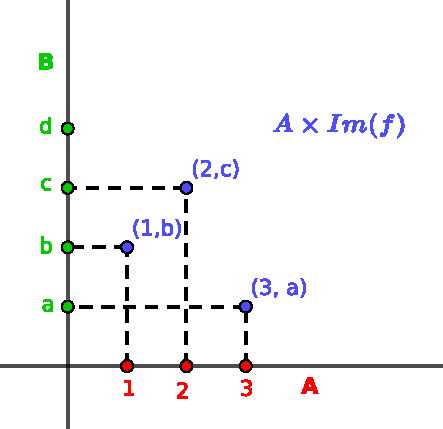
\includegraphics[width=7cm]{./cap_funcao/figs/Grf}}
    \caption{Gráfico da função $f$}
  \end{figure}

\end{exem}


\subsection{Propriedades}
As funções são classificadas em:

\begin{itemize}
 \item \textbf{Injetora}

 Uma função $f: A \rightarrow B$ é injetiva, ou injetora quando:
\begin{equation}
 x_1 \neq x_2 \in A \Rightarrow f(x_1) \neq f(x_2) \in B ,
\end{equation}
 ou equivalentemente usando a contrapositiva:
\begin{equation}
f(x_1) = f(x_2) \in B \Rightarrow x_1 = x_2 .
\end{equation}
 Ou seja, quando cada elemento da $Im(f)$ recebe um único elemento de $A= Dom(f)$, neste caso pode ocorrer de alguns elementos de $B$ não serem imagem de nenhum elemento de $A$ pela função $f$.

 \item \textbf{Sobrejetora}

 Uma função $f: A \rightarrow B$ é sobrejetiva, ou sobrejetora quando para todo $y \in B$, existe pelo menos um elemento $x \in A$ tal que $f(x) = y$. Equivalentemente em símbolos:
\begin{equation}
\forall y \in B, \exists x \in A \text{ tal que } f(x) = y
\end{equation}
 Ou ainda, quando cada elemento de $B$ recebe algum elemento de $A$, neste caso podendo não ser único.

 \item \textbf{Bijetora}

 Uma função $f: A \rightarrow B$ é bijetora, ou bijetiva quando for simultaneamente injetora e sobrejetora. Neste caso, $f$ admite uma inversa que é denotada por $f^{(-1)}$.

\end{itemize}

\begin{multicols}{2}
 \begin{tikzpicture}
 \node (1) at (0,0) {1};%\filldraw(1.east) circle (1pt)
 \node (2) [below of=1] {2};%\filldraw(2.east) circle (1pt)
 \node (3) [below of=2] {3};%\filldraw(3.east) circle (1pt)
 \node[fit=(1) (2) (3),ellipse,draw=red,minimum width=1cm,thick,label=below:\(A\)]{};

 \node (a) at (3,0) {a};%\filldraw($b_1$.west) circle (1pt)
 \node (b) [below of=a] {b};%\filldraw($b_2$.west) circle (1pt)
 \node (c) [below of=b] {c};%\filldraw($b_3$.west) circle (1pt)
 \node[fit=(a) (b) (c),ellipse,draw=green,minimum width=1cm,thick,label=below:\(B\)]{};

 \draw[->, shorten >=.1cm, >=stealth'] (1.east) to (c.west);
 \draw[->, shorten >=.1cm, >=stealth'] (2.east) to (b.west);
 \draw[->, shorten >=.1cm, >=stealth'] (3.east) to (a.west);
\end{tikzpicture} \\
 \textbf{bijetora}\\
 \begin{tikzpicture}
 \node (1) at (0,0) {1};%\filldraw(1.east) circle (1pt)
 \node (2) [below of=1] {2};%\filldraw(2.east) circle (1pt)
 \node (3) [below of=2] {3};%\filldraw(3.east) circle (1pt)
 \node[fit=(1) (2) (3),ellipse,draw=red,minimum width=1cm,thick,label=below:\(A\)]{};

 \node (a) at (3,0) {a};%\filldraw($b_1$.west) circle (1pt)
 \node (b) [below of=a] {b};%\filldraw($b_2$.west) circle (1pt)
 \node[fit=(a) (b),ellipse,draw=green,minimum width=1cm,thick,label=below:\(B\)]{};

 \draw[->, shorten >=.1cm, >=stealth'] (1.east) to (a.west);
 \draw[->, shorten >=.1cm, >=stealth'] (2.east) to (a.west);
 \draw[->, shorten >=.1cm, >=stealth'] (3.east) to (b.west);
\end{tikzpicture} \\
\textbf{sobrejetora e não injetora}
\end{multicols}

\begin{multicols}{2}
 \begin{tikzpicture}
 \node (1) at (0,0) {1};%\filldraw(1.east) circle (1pt)
 \node (2) [below of=1] {2};%\filldraw(2.east) circle (1pt)
 \node (3) [below of=2] {3};%\filldraw(3.east) circle (1pt)
 \node[fit=(1) (2) (3),ellipse,draw=red,minimum width=1cm,thick,label=below:\(A\)]{};

 \node (a) at (3,0) {a};%\filldraw($b_1$.west) circle (1pt)
 \node (b) [below of=a] {b};%\filldraw($b_2$.west) circle (1pt)
 \node (c) [below of=b] {c};%\filldraw($b_3$.west) circle (1pt)
 \node[fit=(a) (b) (c),ellipse,draw=green,minimum width=1cm,thick,label=below:\(B\)]{};

 \draw[->, shorten >=.1cm, >=stealth'] (1.east) to (b.west);
 \draw[->, shorten >=.1cm, >=stealth'] (2.east) to (b.west);
 \draw[->, shorten >=.1cm, >=stealth'] (3.east) to (a.west);
\end{tikzpicture} \\
\textbf{não sobrejetora e não injetora}\\
 \begin{tikzpicture}
 \node (1) at (0,0) {1};%\filldraw(1.east) circle (1pt)
 \node (2) [below of=1] {2};%\filldraw(2.east) circle (1pt)
 \node (3) [below of=2] {3};%\filldraw(3.east) circle (1pt)
 \node[fit=(1) (2) (3),ellipse,draw=red,minimum width=1cm,thick,label=below:\(A\)]{};

 \node (a) at (3,0) {a};%\filldraw($b_1$.west) circle (1pt)
 \node (b) [below of=a] {b};%\filldraw($b_2$.west) circle (1pt)
 \node (c) [below of=b] {c};%\filldraw($b_3$.west) circle (1pt)
 \node (d) [below of=c] {d};%\filldraw($b_3$.west) circle (1pt)
 \node[fit=(a) (b) (c) (d),ellipse,draw=green,minimum width=1cm,thick,label=below:\(B\)]{};

 \draw[->, shorten >=.1cm, >=stealth'] (1.east) to (b.west);
 \draw[->, shorten >=.1cm, >=stealth'] (2.east) to (c.west);
 \draw[->, shorten >=.1cm, >=stealth'] (3.east) to (a.west);
\end{tikzpicture} \\
\textbf{não sobrejetora e injetora}
\end{multicols}

\begin{exem}

 \begin{enumerate}
  \item $f: \mathbb{R} \rightarrow \mathbb{R}$ tal que $f(x) = x^2$

  Neste caso, $f$ não é sobrejetora, nem injetora.

  \begin{dem}

   \begin{itemize}
    \item Sobrejetora

    $f$ não é sobrejetora porque $x^2 \geq 0$, $\forall x \in \mathbb{R}$, logo se considerarmos $y < 0 \in \mathbb{R}$ teremos que $\nexists x \in \mathbb{R}$ tal que $f(x)= y$. Portanto $f$ não é sobrejetora.
    \fim
    \item Injetora

     Note que $ \forall x \in \mathbb{R} \Rightarrow -x \in \mathbb{R}$ e que
\begin{equation}
f(-x)= (-x)^2 = (-x)*(-x) = (x)*(x) = x^2 = f(x)
\end{equation}
    o que mostra que $f$ não é injetora.

   \end{itemize}
  \end{dem}

  \item $f: \mathbb{R_{+}} \rightarrow \mathbb{R}$ tal que $f(x) = x^2$

  Neste caso, $f$ não é sobrejetora, mas é injetora.

  \begin{dem}
   \begin{itemize}
    \item Sobrejetora

    $f$ não é sobrejetora porque $x^2 \geq 0$, $\forall x \in \mathbb{R}$, logo se considerarmos $y < 0 \in \mathbb{R}$ teremos que $\nexists x \in \mathbb{R}$ tal que $f(x)= y$. Portanto $f$ não é sobrejetora.
    \fim
    \item Injetora

    Tome $x_1=x_2 \in \mathbb{R_{+}}$ qualquer, como
\begin{equation}
x_1=x_2 \Rightarrow x_1^2=x_2^2 \Rightarrow f(x_1)=f(x_2)
\end{equation}
    logo $f$ é injetora.

   \end{itemize}
  \end{dem}

  \item $f: \mathbb{R} \rightarrow \mathbb{R_{+}}$ tal que $f(x) = x^2$

  Neste caso, $f$ é sobrejetora, mas não é injetora.

  \begin{dem}
   \begin{itemize}
    \item Sobrejetora

    Tome $y \in \mathbb{R_{+}}$ qualquer, como $y \geq 0$ existe $x \in \mathbb{R}$ tal que
\begin{equation}
x = \sqrt{y} \Rightarrow x^2 = (\sqrt{y})^2 \Rightarrow x^2 = y \Rightarrow f(x) = y 
\end{equation}
    portanto $f$ é sobrejetora.
    \fim
    \item Injetora

    Note que $ \forall x \in \mathbb{R} \Rightarrow -x \in \mathbb{R}$ e que
\begin{equation}
f(-x)= (-x)^2 = (-x)*(-x) = (x)*(x) = x^2 = f(x)
\end{equation}
    o que mostra que $f$ não é injetora.

   \end{itemize}
  \end{dem}

  \item $f: \mathbb{R_{+}} \rightarrow \mathbb{R_{+}}$ tal que $f(x) = x^2$ ou $f: \mathbb{R_{-}} \rightarrow \mathbb{R_{+}}$ tal que $f(x) = x^2$

  Neste caso, $f$ é sobrejetora, e é injetora, portanto bijetora.

  \begin{dem}
   \begin{itemize}
    \item Sobrejetora

    Tome $y \in \mathbb{R_{+}}$ qualquer, como $y \geq 0$ existe $x \in \mathbb{R}$ tal que
\begin{equation}
x = \sqrt{y} \Rightarrow x^2 = (\sqrt{y})^2 \Rightarrow x^2 = y \Rightarrow f(x) = y
\end{equation}
    portanto $f$ é sobrejetora.
    \fim
    \item Injetora

    Tome $x_1, x_2 \in \R_{+}$, tais que $f(x_1) = f(x_2)$ logo,
\begin{equation}
f(x_1) = f(x_2) \Rightarrow x_1^2= x_2^2 \Rightarrow \sqrt{x_1^2}= \sqrt{x_2^2} \Rightarrow \abs{x_1}= \abs{x_2} \Rightarrow x_1= x_2, 
\end{equation}
    pois $x_1, x_2 \geqslant 0$. Portanto $f$ é injetora.

   \end{itemize}
  \end{dem}

 \end{enumerate}

\end{exem}

\subsection{Operações com funções}
Dadas as funções $f: A \rightarrow \R$, $g: B \rightarrow \R$, se $A \cap B \neq \emptyset$, então $\forall x \in A \cap B$, definimos as seguintes operações entre estas funções:
\begin{equation}
(f + g)(x)= f(x) + g(x); 
\end{equation}
\begin{equation}
(f - g)(x)= f(x) - g(x); 
\end{equation}
\begin{equation}
(f \cdot g)(x)= f(x) \cdot g(x); 
\end{equation}
\begin{equation}
 \left( \frac{f}{g} \right) (x)= \frac{f(x)}{g(x)} ;
\end{equation}
\begin{equation}
(k \cdot f)(x)= k \cdot f(x), \text{ para } k \text{ constante} ,
\end{equation}

note que:
\begin{equation}
dom(f+g)= dom(f-g)= dom(f \cdot g)= dom(k \cdot f)= A \cap B ,
\end{equation}
\begin{equation}
 dom\left( \frac{f}{g} \right)= \{x \in A \cap B \mid g(x) \neq 0\}. 
\end{equation}

Além destas operações, é possível também definir a composição de funções. Para isso consideremos duas funções $f: A \rightarrow B$ e $g: C \rightarrow D$, com $A, B, C \text{ e } D \subset \R$, e tais que $Im(f) \subset C$ , assim a função composta $g \circ f: A \rightarrow D$ é definida por:
\begin{equation}
(g \circ f)(x)= g(f(x)). 
\end{equation}

\section{Tipos de funções}

\subsection{Função constante}

É a função que associa todos os elementos do domínio a um único elemento do contradomínio. Ou seja, dado $a \in \R$ fixo, a função $f$:
\begin{eqnarray*}
 f: \R & \rightarrow & \R \\
 x & \mapsto & a,
\end{eqnarray*}
é uma função constante.

Por exemplo, a função $f$:
\begin{eqnarray*}
 f: \R & \rightarrow & \R \\
 x & \mapsto & 2 \ .
\end{eqnarray*}

É uma função constante. Para construir o gráfico desta função começamos encontrando alguns pontos $(x, y)= (x, f(x))$ do gráfico, o que pode ser feito através da seguinte tabela:

 \begin{table}[H]
 \centering
 \begin{tabular}{|c|c|c|} \hline
 \rowcolor{cinza}
  x & f(x)= 2 & (x, y)  \\\hline
  -1 & f(-1)= 2 & (-1, 2) \\\hline
   0 & f(0)= 2 & (0, 2)  \\\hline
   1 & f(1)= 2 & (1, 2) \\\hline
 \end{tabular}
\end{table}

Após encontrar os pontos basta marcar os mesmo o plano cartesiano e traçar a curva que liga estes pontos com isso objetos o gráfico da função. Neste caso o gráfico é:
\begin{figure}[H]
 \centering
    \fbox{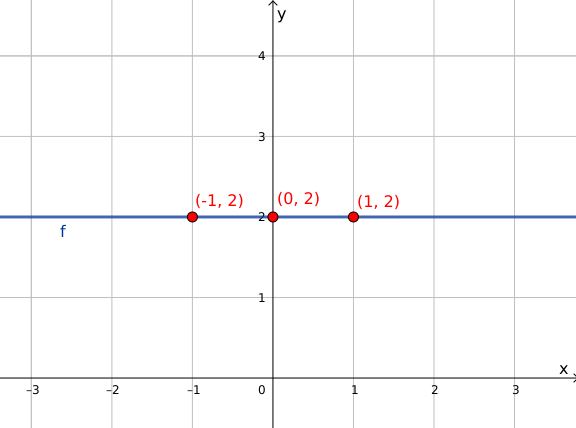
\includegraphics[width=7cm]{./cap_funcao/figs/f(x)=2}}
    \caption{Gráfico da função $f(x)=2$}
  \end{figure}

\subsection{Função identidade}

A função $Id$:
\begin{eqnarray*}
 Id: \R & \rightarrow & \R \\
 x & \mapsto & x \ ,
\end{eqnarray*}
é chamada \textit{função identidade real}.

Para encontrar alguns pontos $(x, f(x))$ do gráfico desta função, construímos a seguinte tabela:

 \begin{table}[H]
 \centering
 \begin{tabular}{|c|c|c|} \hline
 \rowcolor{cinza}
  x & f(x)= x & (x, y)  \\\hline
  -1 & f(-1)= -1 & (-1, -1) \\\hline
   0 & f(0)= 0 & (0, 0)  \\\hline
   1 & f(1)= 1 & (1, 1) \\\hline
 \end{tabular}
\end{table}

Logo o gráfico da função $Id$ é:
\begin{figure}[H]
 \centering
    \fbox{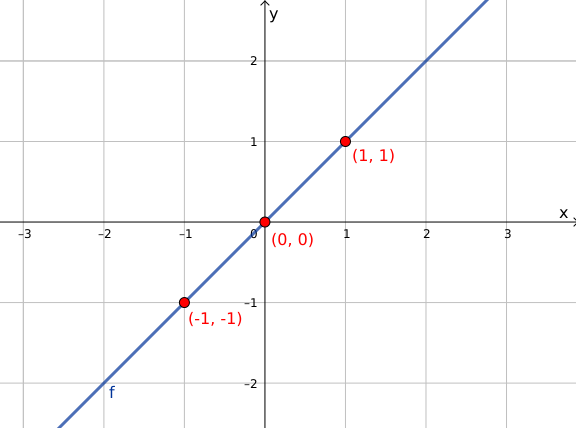
\includegraphics[width=7cm]{./cap_funcao/figs/Id(x)=x}}
    \caption{Gráfico da função $Id(x)=x$}
  \end{figure}


\subsection{Funções polinomiais de grau \texorpdfstring{$n$}{n}}

 \vskip0.3cm
 \colorbox{azul}{
 \begin{minipage}{0.9\linewidth}
 \begin{center}
 As funções $f: \R \to \R$ com a seguinte regra geral:
\begin{equation}
f(x) = a_0 + a_1 x + a_2 x^2 + a_3 x^3 + \cdots + a_n x^n
\end{equation}
 para $\{a_0, a_1, a_2, a_3, \ldots a_n\} \in \R$ e $n \in \N$, tais que $a_n \neq 0$ são denominadas \\ \textbf{funções polinomiais de grau $n$}.
 \end{center}
 \end{minipage}}
 \vskip0.3cm



 Casos particulares:
 \begin{itemize}
 \item Funções do 1º grau, ou funções afim

 São funções $f: \R \rightarrow \R$ dadas por:
\begin{equation}
f(x)= ax + b \ , 
\end{equation}

 para certos $a, b \in \R$ com $a \neq 0$. Note que um caso particular e já conhecido de função de 1º grau é a função identidade, $f(x)= x$, a qual possui $a=1$ e $b=0$.

 Vejamos mais alguns exemplos de funções de 1º grau.

 Consideremos as funções $f, g: \R \to \R$ dadas por:
 \begin{enumerate}[a)]
  \item $f(x)= x+2$
  \item $g(x)= x-1$
 \end{enumerate}


 \begin{figure}[H]
   \fbox{\subfigure[$f(x)= x+2$]{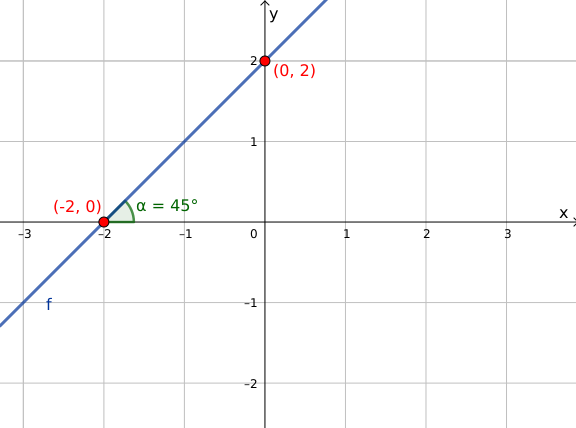
\includegraphics[width=7cm,height=6cm]{./cap_funcao/figs/f(x)=x+2}}}
   \fbox{\subfigure[$g(x)= x-1$]{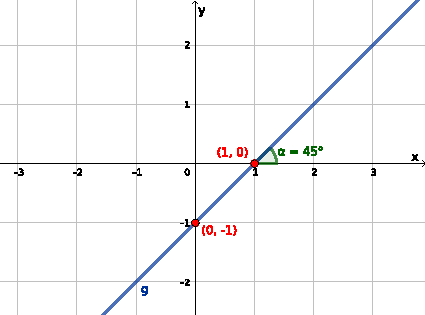
\includegraphics[width=7cm,height=6cm]{./cap_funcao/figs/f(x)=x-1}}}
  \end{figure}
  Note que o que muda na definição destas funções é apenas o coeficiente $b$. Fazendo uma análise comparativa dos gráficos destas funções notamos que os ângulos que as retas formam com o eixo $x$ é o mesmo, portanto as retas são paralelas, porém o ponto de interseção das retas com o eixo $y$, que são os pontos $(0, f(0))$, $(0, g(0))$ muda, ou seja, $f(0) \neq g(0)$. De fato:
\begin{equation}
f(0)= 0 + 2= 2
\end{equation}
\begin{equation}
g(0)= 0 -1 = -1 \ .
\end{equation}
  No caso geral em que $f(x)=ax+b$, teremos que $f(0)=a0 + b= b$, portanto o gráfico de $f$ irá intersectar o eixo $y$ no ponto $(0,b)$. O coeficiente $b$ é chamado de \textbf{coeficiente linear} da reta/função linear.

  Consideremos as funções $f, g: \R \to \R$ dadas por:
 \begin{enumerate}[a)]
  \item $f(x)= 2x$
  \item $g(x)= -2x$
 \end{enumerate}

 \begin{figure}[H]
   \fbox{\subfigure[$f(x)= 2x$]{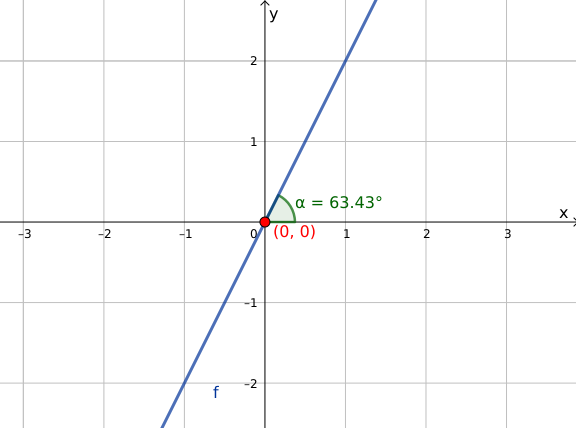
\includegraphics[width=7cm,height=6cm]{./cap_funcao/figs/f(x)=2x}}}
   \fbox{\subfigure[$g(x)= -2x$]{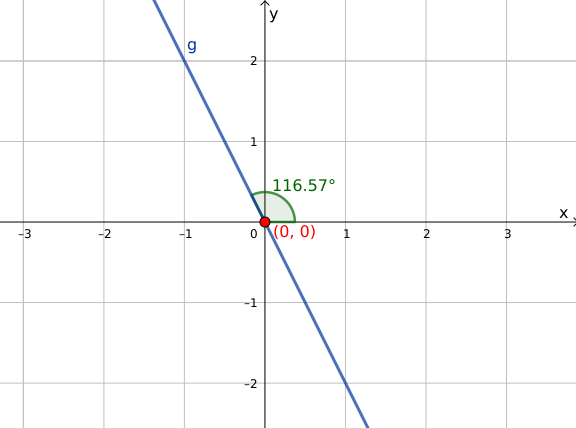
\includegraphics[width=7cm,height=6cm]{./cap_funcao/figs/g(x)=-2x}}}
  \end{figure}
  Neste exemplos estamos mudando apenas o coeficiente $a$ das funções, o que está alterando o ângulo que as retas formam com o eixo $x$, ou seja a inclinação das retas em relação ao eixo $x$. Já o ponto de interseção das retas com o eixo $y$ é o mesmo pois $f(0)= g(0)= 0$. O coeficiente $a$ é chamado de \textbf{coeficiente angular} da reta/função linear.

   \vskip0.3cm
 \colorbox{amarelo}{
 \begin{minipage}{0.9\linewidth}
 \begin{center}
 O gráfico de uma função linear $f: \R \to \R$ dada por:
\begin{equation}
f(x) = ax + b
\end{equation}
 é uma reta com coeficiente angular $a$ e cuja interseção com o eixo $y$ ocorre no ponto $(0, b)$.
 \end{center}
 \end{minipage}}
 \vskip0.3cm

 Frequentemente a equação da reta é dada pela equação $y=mx+n$, que nada mais é do que uma função de 1º grau, basta considerar $y=f(x)$ o que fazemos no contexto de funções para trabalhar com o gráfico da função.

 \textbf{Coeficiente angular da reta}

  Dados dois pontos $P_0=(x_0, y_0)$, $P_1=(x_1, y_1)$, com $x_0 \neq x_1$, como na figura:

 \begin{figure}[H]
 \centering
    \fbox{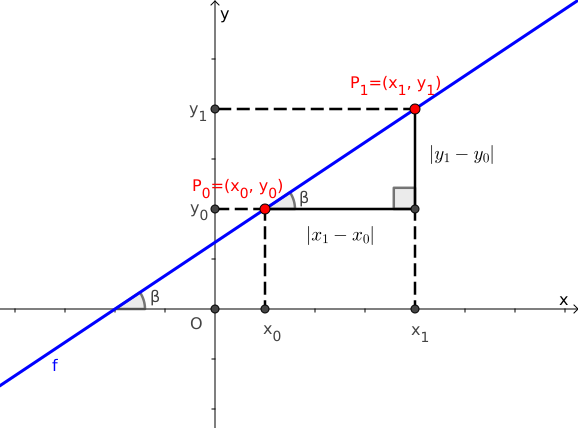
\includegraphics[width=8cm]{./cap_funcao/figs/coefangular}}
    \caption{Coeficiente angular}
  \end{figure}

  o coeficiente angular da reta que passa por estes dois pontos é dado por:
\begin{equation}
a= \frac{y_1 - y_0}{x_1 - x_0} \ \ \ \text{ ou } \ \ \ a= \frac{y_0 - y_1}{x_0 - x_1} \ .
\end{equation}

  De fato, dados dois pontos $P_0=(x_0, y_0)$, $P_1=(x_1, y_1)$, com $x_0 \neq x_1$, podemos encontrar a função $f(x)= ax+b$, cujo gráfico passa por estes dois pontos lembrando que ambos devem satisfazer a equação da função assim obtemos:
  \[ \begin{cases}
   y_0= ax_0 + b \\
   y_1= ax_1 + b
  \end{cases} \]
  logo $y_0 - ax_0= b$, substituindo na segunda equação decorre que:
\begin{equation}
y_1= ax_1 + y_0 - ax_0 \Rightarrow y_1 - y_0= a(x_1 - x_0) \Rightarrow a= \frac{y_1 - y_0}{x_1 - x_0} \ . 
\end{equation}

  Este sistema linear sempre pode ser usado para encontrar a regra da função linear que passa por dois pontos dados.


  \begin{exem}
  Vamos determinar o coeficiente angular da reta que passa pelos pontos:
   \begin{enumerate}[a)]
    \item $P_0=(0,2)$ e $P_1=(-2,0)$
\begin{equation}
a= \frac{y_1 - y_0}{x_1 - x_0}= \frac{0 - 2}{-2 - 0}= \frac{-2}{-2}= 1
\end{equation}
    \item $P_0=(1,2)$ e $P_1=(-1,-2)$
\begin{equation}
a= \frac{y_1 - y_0}{x_1 - x_0}= \frac{-2 - 2}{-1 - 1}= \frac{-4}{-2}= 2
\end{equation}
   \end{enumerate}

  \end{exem}

  Quando dados dois pontos $P_0=(x_0, y_0)$, $P_1=(x_1, y_1)$, com $x_0 = x_1$, temos uma reta vertical, cuja equação é $x= a$ para algum $a \in \R$, que não é o gráfico de uma função, por isso não iremos detalhar este caso.

  Dadas duas funções lineares $f(x)=a_1 x + b_1$ e $g(x)= a_2 x + b_2$, tais que $f(x) \neq g(x)$, a partir da análise de seus coeficientes angulares podemos conhecer a posição relativa de seus gráficos. Nesta situação temos que dois casos especiais:
  \begin{itemize}
  \item Se $a_1= a_2$ então os gráficos de $f$ e $g$ são retas \textbf{paralelas};
  \item Se $a_1 \cdot a_2= -1$ então os gráficos de $f$ e $g$ são retas \textbf{perpendiculares}.
  \end{itemize}

  \begin{exem}
  Considere as funções $g(x)= -2x+4$, $f(x)= -2x+2$, $h(x)= \frac{-1}{-2}x+ 1,5$, pela análise com coeficientes angulares temos que os gráficos de $g$ e $f$ são retas paralelas e os gráficos $g$ e $h$ são retas perpendiculares, como podemos ver nos seguintes gráficos:
     \begin{figure}[H]
   \fbox{\subfigure[Retas paralelas]{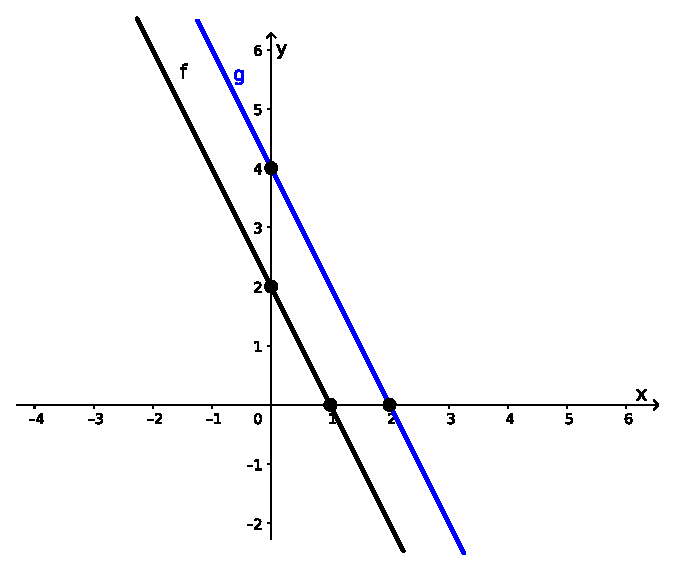
\includegraphics[width=7cm,height=6cm]{./cap_funcao/figs/retasparalelas}}}
   \fbox{\subfigure[Retas perpendiculares]{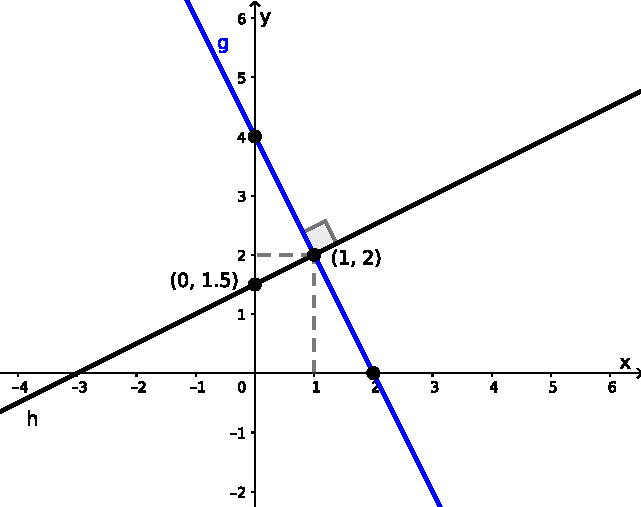
\includegraphics[width=7cm,height=6cm]{./cap_funcao/figs/retasperpendiculares}}}
  \end{figure}
  \end{exem}



 \textbf{Zeros ou raízes das funções lineares}

 \vskip0.3cm
 \colorbox{azul}{
 \begin{minipage}{0.9\linewidth}
 \begin{center}
 Os zeros ou raízes de uma função $y= f(x)$ são os $x \in Dom(f)$ tais que $f(x)= 0$.
 \end{center}
 \end{minipage}}
 \vskip0.3cm

 Desta definição de \textbf{zeros} decorre que os zeros de uma função de 1º grau são as raízes da equação $ax+b=0$. Como esta equação é do 1º grau, ela possui uma única raiz, logo a função de 1º grau também possui uma única raiz, que denotaremos por $\tilde{x}$. Note que o ponto $(\tilde{x}, 0) \in \R^2$ é o ponto de interseção do gráfico da $f$ com o eixo $x$, assim podemos interpretar graficamente as raízes da nossa função como sendo os pontos de interseção do gráfico da função com o eixo das abscissas.

 \item Funções do 2º grau ou função quadrática

 São funções $f: \R \rightarrow \R$ dadas por:
\begin{equation}
f(x)= ax^2 + bx + c
\end{equation}

 Os \textbf{zeros} ou \textbf{raízes} das funções de 2º grau $f$, quando existem, são os $x \in dom(f)$ tais que $ax^2+bx+c=0$. Por ser esta uma equação do 2º grau temos três situações a considerar, dependendo do valor de $\Delta$:
 
 \destaque{\Delta= b^2 - 4*a*c}

 Se \destaque{\Delta < 0} a função $f$ não possui raízes reais;

 Se \destaque{\Delta = 0} a função $f$ possui uma única raiz real;

 Se \destaque{\Delta > 0} a função $f$ possui duas raízes reais distintas, que podem ser calculadas resolvendo a equação de 2º grau através da fórmula para equações de 2º grau.

 Por definição, os zeros da função $f(x)= ax^2+bx+c$, são as raízes da equação $ax^2+bx+c=0$, já que estes são os valores de $x$ para os quais $f(x)=0$. Graficamente, quando estas funções possuem zeros eles são exatamente os pontos de interseção do gráfico da $f$ com o eixo $x$.

 Com relação a concavidade, o gráfico da função de 2º grau tem concavidade voltada \textbf{para cima} quando \destaque{a > 0}, e concavidade voltada \textbf{para baixo} quando \destaque{a < 0}.

 Em ambos os casos a função do 2º grau possui um vértice dado pela seguinte equação:

 \destaque{V= \left(\frac{- b}{2a}, \frac{- \Delta}{4a} \right)}.

 No caso em que $a > 0$, o vértice do gráfico da função de 2º grau é um ponto de mínimo da função.

 No caso em que $a < 0$, o vértice do gráfico da função de 2º grau é um ponto de máximo da função.


  \begin{figure}[H]
   \fbox{\subfigure[$a > 0$ e $\Delta < 0$]{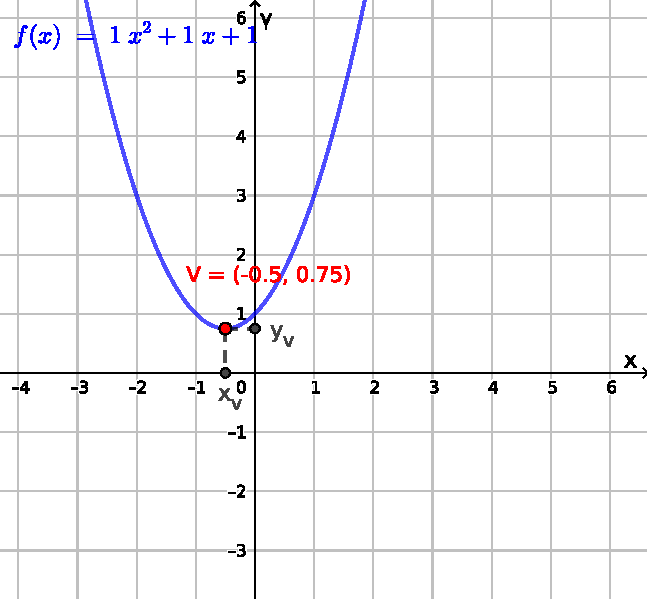
\includegraphics[width=7cm,height=6cm]{./cap_funcao/figs/f1}}}
   \fbox{\subfigure[$a > 0$ e $\Delta = 0$]{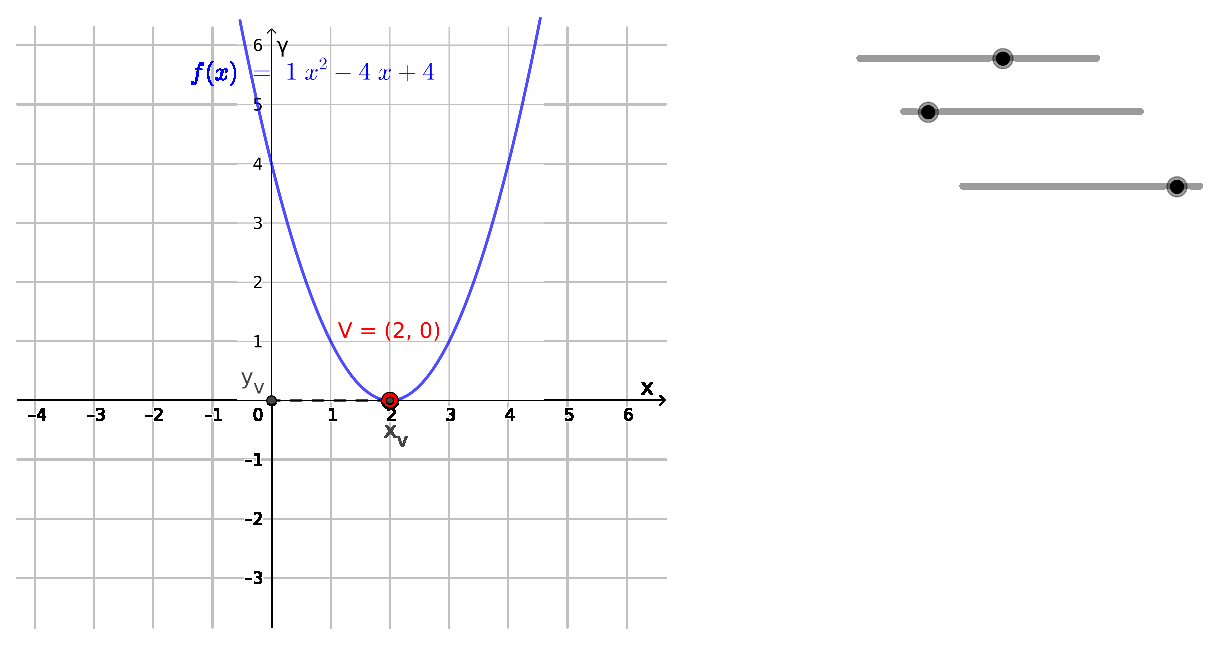
\includegraphics[width=7cm,height=6cm]{./cap_funcao/figs/f2}}}
  \end{figure}

  \begin{figure}[H]
   \fbox{\subfigure[$a > 0$ e $\Delta > 0$]{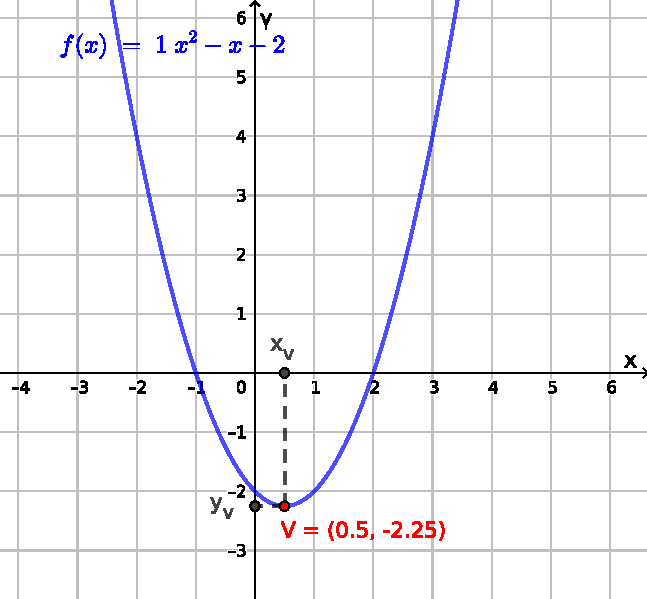
\includegraphics[width=7cm,height=6cm]{./cap_funcao/figs/f3}}}
   \fbox{\subfigure[$a < 0$ e $\Delta < 0$]{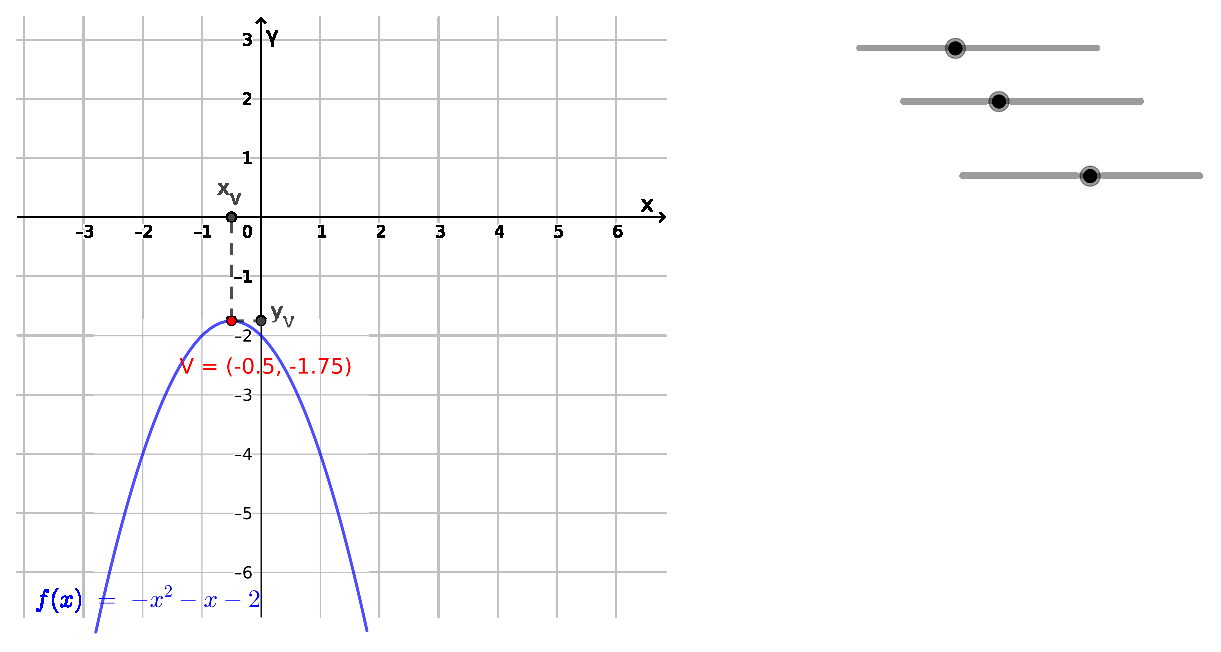
\includegraphics[width=7cm,height=6cm]{./cap_funcao/figs/f4}}}
  \end{figure}

   \begin{figure}[H]
   \fbox{\subfigure[$a < 0$ e $\Delta = 0$]{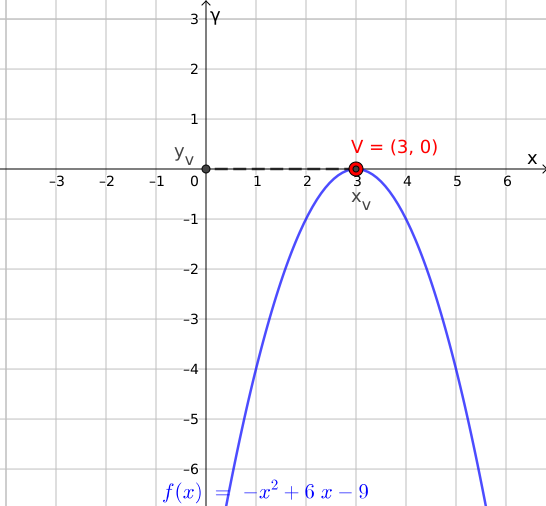
\includegraphics[width=7cm,height=6cm]{./cap_funcao/figs/f5}}}
   \fbox{\subfigure[$a < 0$ e $\Delta > 0$]{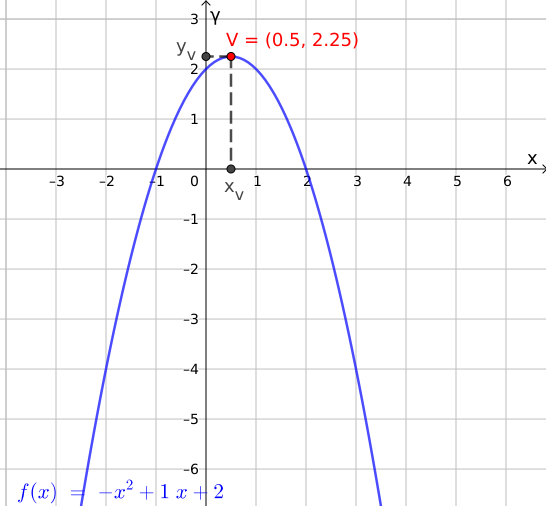
\includegraphics[width=7cm,height=6cm]{./cap_funcao/figs/f6}}}
   \caption{Gráficos de funções do 2º grau}
 \end{figure}


 \newpage
 \item Funções do 3º grau ou funções cúbicas

 São funções $f: \R \rightarrow \R$ dadas por:
\begin{equation}
f(x)= ax^3 + bx^2 + cx + d .
\end{equation}

 As \textbf{raízes} ou \textbf{zeros} das funções de 3º grau são os $x \in \R$ tais que $ax^3 + bx^2 + cx + d=0$. Assim as funções de 3º grau podem classificadas de acordo com suas raízes em 4 casos:
 \begin{enumerate}[(I)]
  \item 3 raízes reais distintas;
  \item 1 raiz real e duas raízes complexas;
  \item 3 raízes reais sendo duas delas iguais;
  \item 3 raízes reais iguais.
 \end{enumerate}
 Estes casos estão representados nos gráficos abaixo, onde consideramos sempre $a< 0$, o caso $a> 0$ é análogo.


   \begin{figure}[H]
   \fbox{\subfigure[$a < 0$]{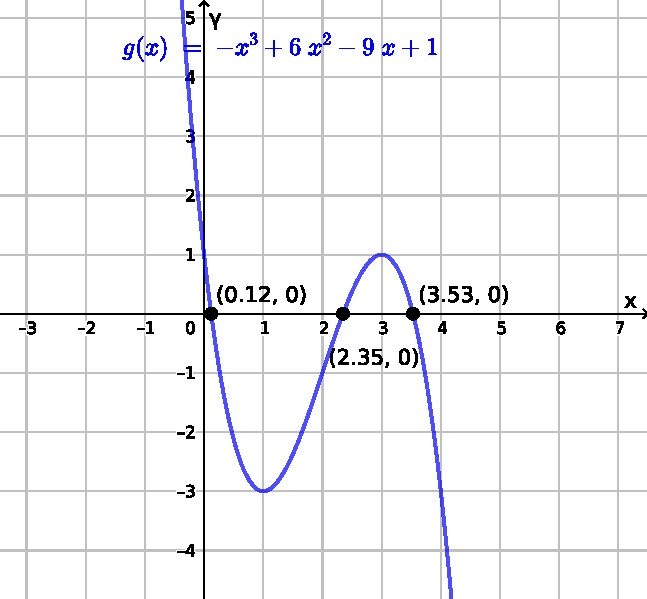
\includegraphics[width=7cm,height=5cm]{./cap_funcao/figs/g1}}}
   \fbox{\subfigure[$a < 0$]{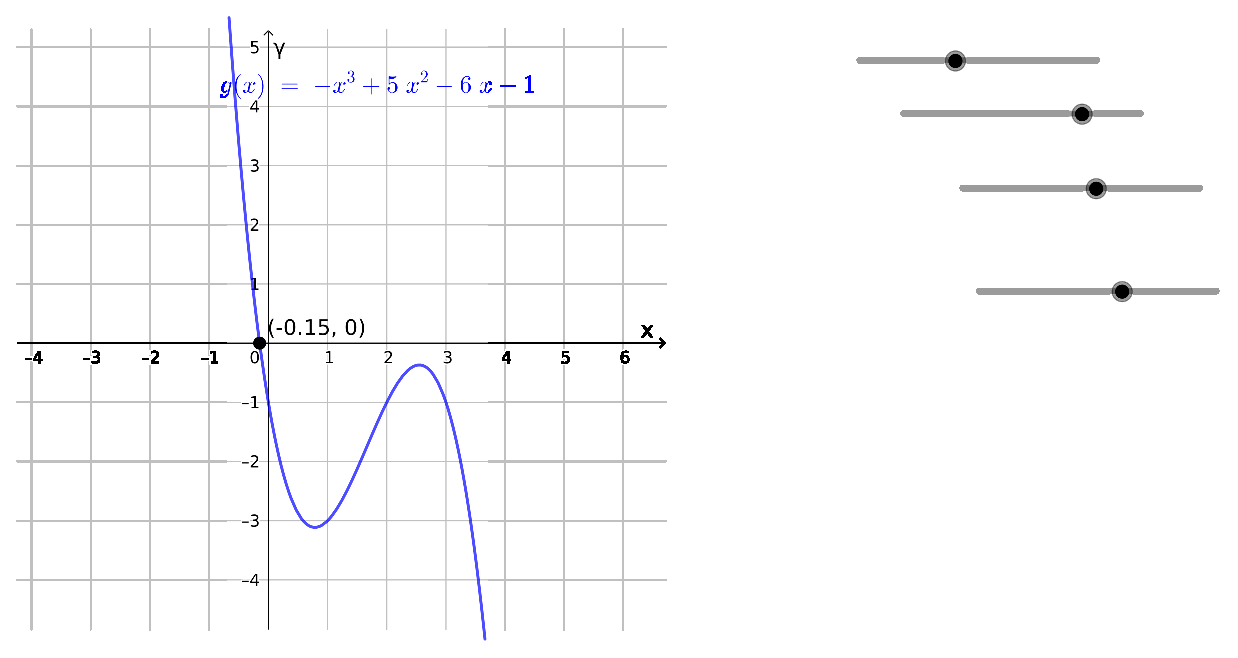
\includegraphics[width=7cm,height=5cm]{./cap_funcao/figs/g2}}}
   \end{figure}

  \begin{figure}[H]
   \fbox{\subfigure[$a < 0$]{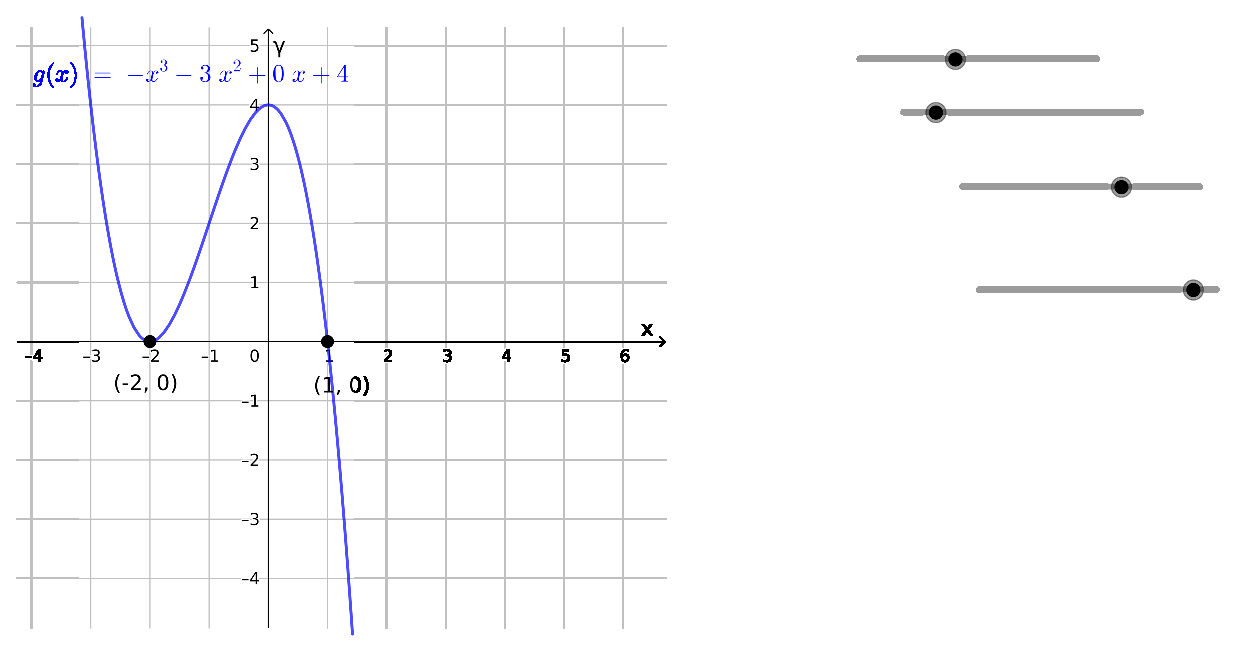
\includegraphics[width=7cm,height=5cm]{./cap_funcao/figs/g3}}}
   \fbox{\subfigure[$a < 0$]{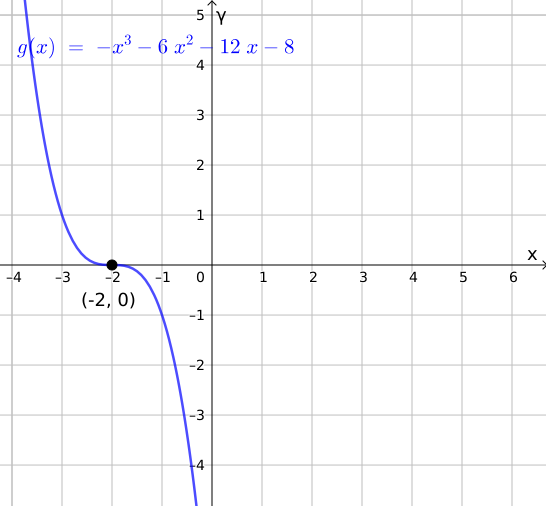
\includegraphics[width=7cm,height=5cm]{./cap_funcao/figs/g4}}}
   \caption{Gráficos de funções do 3º grau}
  \end{figure}

 \end{itemize}


  \subsection{Função modular}

  Considere a função $f: \R \rightarrow \R$, dada por $f(x)= \abs{x}$, pela definição de módulo temos que $f$ é uma função definida por partes, da seguinte forma:

  \[f(x)= \abs{x} = \begin{cases}
                 x, \text{ se } x \geq 0 \\
                 -x, \text{ se } x < 0
                \end{cases} \ .\]

 Cujo gráfico é dado por:

  \begin{figure}[H]
 \centering
    \fbox{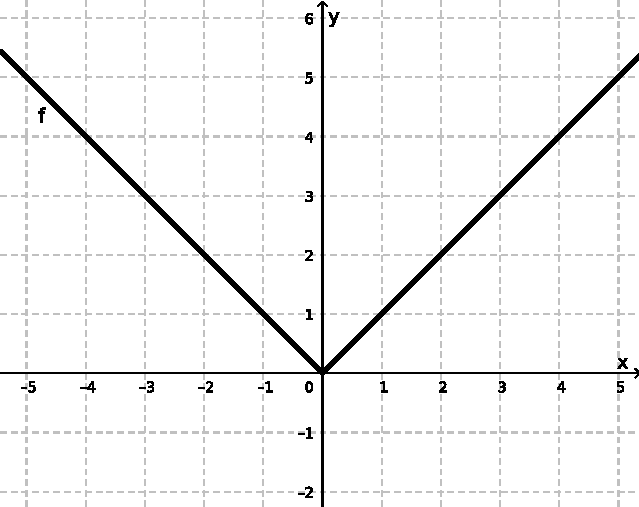
\includegraphics[width=8cm]{./cap_funcao/figs/funcaomodulo}}
    \caption{Gráfico da função módulo}
  \end{figure}

  Note que $f$ é decrescente no intervalo $]-\infty, 0[$, e crescente no intervalo $]0, \infty[$, e admite um mínimo em $x=0$.

  Consideramos agora a função $f_1: \R \rightarrow \R$ dada por $f_1(x)= \abs{x+1}$, observe que:
\begin{equation}
x+1 \geq 0 \Leftrightarrow  x \geq -1
\end{equation}
  com isso podemos reescrever a função $f_1$ sem os módulos da seguinte forma:

  \[f_1(x)= \begin{cases}
                 x + 1, \text{ se } x \geq -1 \\
                 -x - 1, \text{ se } x < -1
                \end{cases} \ .\]
  Com isso a função modular pode ser vista como uma função linear por partes.

  Analogamente, para a função $f_2: \R \rightarrow \R$ dada por $f_2(x)= \abs{x+1}+2$, temos que:
\begin{equation}
x+1 \geq 0 \Leftrightarrow  x \geq -1
\end{equation}
  com isso podemos reescrever a função $f_2$ sem os módulos da seguinte forma:

  \[f_2(x)= \begin{cases}
                 x + 3, \text{ se } x \geq -1 \\
                 -x + 1, \text{ se } x < -1
                \end{cases} \ .\]
  Com isso a função modular também pode ser vista como uma função linear por partes.

  Os gráficos das funções $f$, $f_1$ e $f_2$ estão dados na figura a seguir.

  \begin{figure}[H]
 \centering
    \fbox{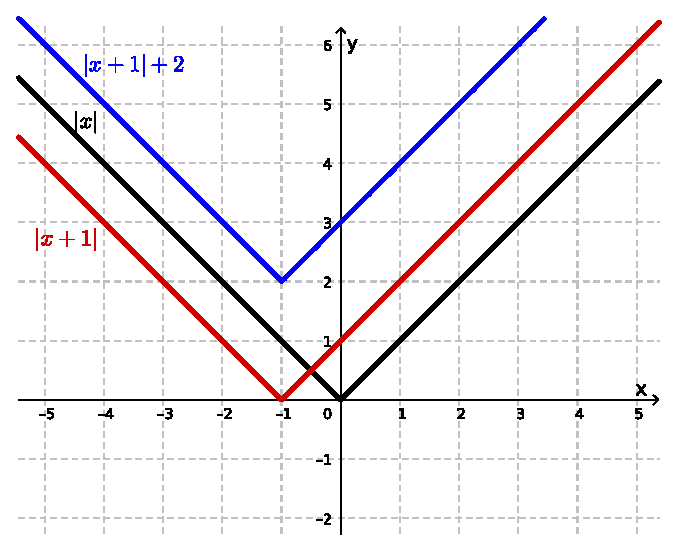
\includegraphics[width=8cm]{./cap_funcao/figs/funcaomodulo2}}
    \caption{Gráfico da função módulo}
  \end{figure}

  Comparando os gráficos das funções $f$ e $f_1$ notamos que ao somar uma constante ``dentro'' do módulo transladamos o gráfico da função $f$ no eixo $x$, e ao comparar as funções $f_1$ e $f_2$ percebemos que ao somar uma constante ``fora'' do módulo fazemos uma translação do gráfico da função $f_1$ em relação ao eixo $y$.

  \subsection{Mais algumas funções interessantes}

  \textbf{Função raiz quadrada}

  É a função $f: \R_{+} \to \R_{+}$ dada por $f(x)= \sqrt{x}$, cujo gráfico é:

   \begin{figure}[H]
 \centering
    \fbox{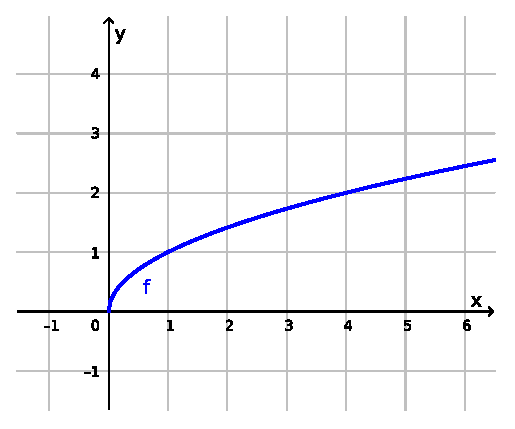
\includegraphics[width=6cm]{./cap_funcao/figs/funcaoraizquadrada}}
    \caption{Função raiz quadrada}
  \end{figure}

  Note que neste caso o domínio da função são apenas os números reais positivos, já que não existe raiz quadrada de número negativo.

  \newpage
  \textbf{Função raiz cúbica}

  É a função $f: \R \to \R$ dada por $f(x)= \sqrt[3]{x}$, cujo gráfico é:

   \begin{figure}[H]
 \centering
    \fbox{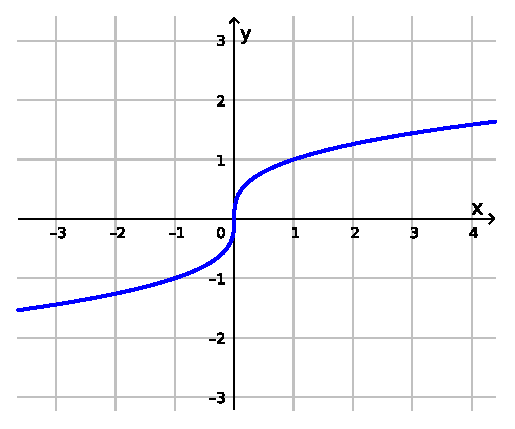
\includegraphics[width=6cm]{./cap_funcao/figs/funcaoraizcubica}}
    \caption{Função raiz cúbica}
  \end{figure}

  \textbf{Função recíproca}

  É a função $f: \R \setminus \{0\} \to \R$ dada por $f(x)= \frac{1}{x}$, cujo gráfico é:

   \begin{figure}[H]
 \centering
    \fbox{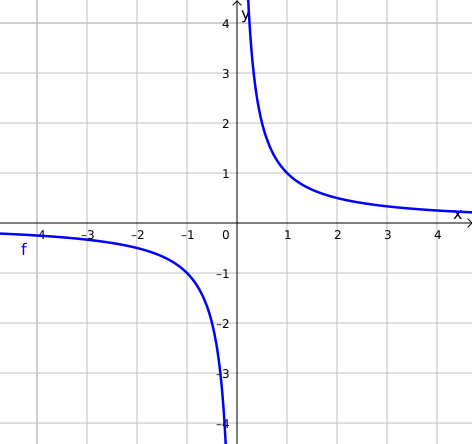
\includegraphics[width=6cm]{./cap_funcao/figs/funcaoreciproca}}
    \caption{Função recíproca}
  \end{figure}

  Neste caso o domínio da função é o conjunto $\R \setminus \{0\}$, pois não existe divisão por $0$ (zero).

  \newpage

  \textbf{Função floor}

  É a função $f: \R \to \R$ dada por $f(x)= \lfloor {x} \rfloor$, cujo gráfico é:

   \begin{figure}[H]
 \centering
    \fbox{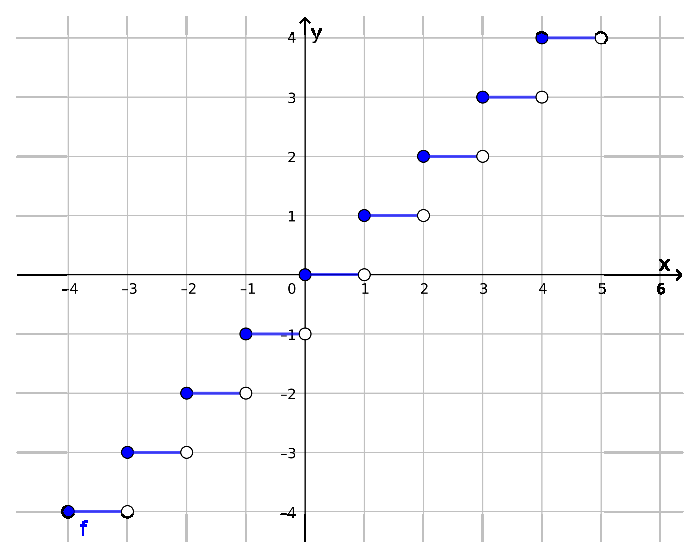
\includegraphics[width=6cm]{./cap_funcao/figs/funcaofloor}}
    \caption{Função floor}
  \end{figure}

  Esta função aplicada em um número $x$ tem como imagem a parte inteira do número $x$.

  \textbf{Função ceil}

  É a função $f: \R \to \R$ dada por $f(x)= \lceil {x} \rceil$, cujo gráfico é:

   \begin{figure}[H]
 \centering
    \fbox{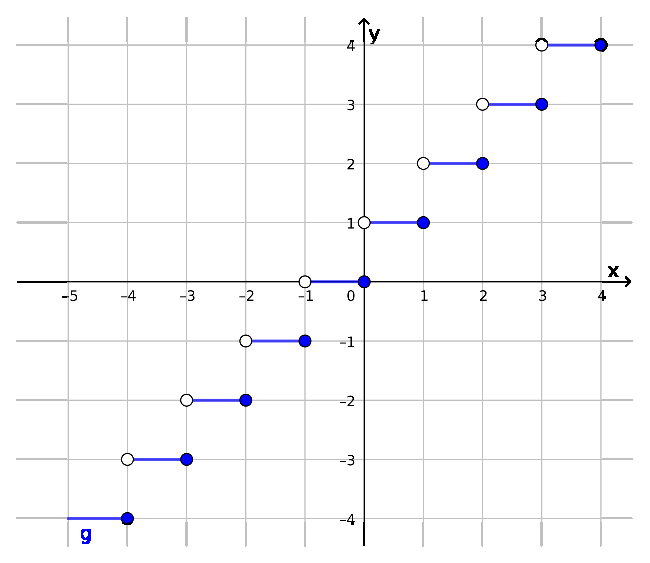
\includegraphics[width=6cm]{./cap_funcao/figs/funcaoceil}}
    \caption{Função ceil}
  \end{figure}

  Esta função aplicada em um número $x$ tem como imagem o menor inteiro maior ou igual a $x$.

  \section{Algumas propriedades das funções}

   \vskip0.3cm
 \colorbox{azul}{
 \begin{minipage}{0.9\linewidth}
 \begin{center}
  Dados $A, B \subset \R$ e uma função $f: A \rightarrow B$.

  Dizemos que $f$ é uma \textbf{função crescente} em um intervalo $I \subset A$ se, para todo $x, y \in I$,
\begin{equation}
 x < y \Rightarrow f(x) < f(y) \ .
\end{equation}
  Dizemos que $f$ é uma \textbf{função decrescente} em um intervalo $I \subset A$ se, para todo $x, y \in I$,
\begin{equation}
x < y \Rightarrow f(x) > f(y) \ .
\end{equation}
  Dizemos que $f$ é uma \textbf{função constante} em um intervalo $I \subset A$ se, para todo $x, y \in I$,
\begin{equation}
x \neq y \Rightarrow f(x) = f(y) \ .
\end{equation}
 \end{center}
 \end{minipage}}
 \vskip0.3cm

 \begin{exem}
 Seja $f: \R \to \R$ uma função dada por $f(x)= ax + b$.

 Quando {a > 0}, dados $x_1 < x_2 \in dom(f)$, temos que:
\begin{equation}
x_1 < x_2 \Rightarrow ax_1 < ax_2 \Rightarrow ax_1 + b < ax_2 + b \ ,
\end{equation}
  portanto $f(x_1) < f(x_2)$, neste caso dizemos que $f$ é \textbf{crescente}.

 Quando \destaque{a < 0}, dados $x_1 < x_2 \in dom(f)$, temos que:
\begin{equation}
x_1 < x_2 \Rightarrow ax_1 > ax_2 \Rightarrow ax_1 + b > ax_2 + b \ ,
\end{equation}
 portanto $f(x_1) > f(x_2)$, neste caso dizemos que $f$ é \textbf{decrescente}.

 Observe que no caso das funções de 1º grau a propriedade de ser crescente ou decrescente é válida em todo o domínio da função, nestes casos dizemos que é uma propriedade global da função.
 \end{exem}

 \begin{exem}
 Vamos retomar alguns dos nossos exemplos de funções para classificar como crescente, decrescente e constante. Para isso considere $x_1= -2$ e $x_2= 1$, neste caso, $x_1 < x_2$.
  \begin{enumerate}[a)]
   \item Sendo $f(x)= \frac{1}{2}x + 1,5$, temos que
\begin{equation}
f(x_1)= f(-2)= \frac{1}{2}\cdot (-2) + 1,5= -1 + 1,5= 0,5
\end{equation}
\begin{equation}
f(x_2)= f(1)= \frac{1}{2} \cdot 1+\frac{3}{2}= \frac{4}{2}= 2
\end{equation}
   logo $f(x_1)= 0,5 < 2= f(x_2)$. Portanto $f$ é crescente.
   \item Sendo $f(x)= -2x + 2$, temos que
\begin{equation}
f(x_1)= f(-2)= -2 \cdot (-2) + 2= 4 + 2= 6
\end{equation}
\begin{equation}
f(x_2)= f(1)= -2 \cdot 1 + 2= 0
\end{equation}
   logo $f(x_1)= 6 > 0 = f(x_2)$. Portanto $f$ é decrescente.
   \item Sendo $f(x)= 2$, temos que
\begin{equation}
f(x_1)= f(-2)= 2
\end{equation}
\begin{equation}
f(x_2)= f(1)= 2
\end{equation}
   logo $f(x_1)= 2 = 2= f(x_2)$. Portanto $f$ é constante.
  \end{enumerate}
  Como já mostramos acima que para as funções lineares esta propriedade é global, para fazer esta classificação é suficiente testar dois valores de $x$ como fizemos acima.

 \end{exem}

 \begin{exem}
  Considere a função $f(x)= \abs{x}$. Lembramos que esta função é definida por partes, por isso faremos a análise de crescimento e decrescimento em cada uma destas partes.

  Caso 1: Se $x < 0$, temos que $f(x)= -x$, logo se $x_1 < x_2$,
\begin{equation}
x_1 < x_2 \Rightarrow -x_1 > -x_2 \Rightarrow f(x_1) > f(x_2) \ ,
\end{equation}
  por exemplo, sendo $x_1= -3$ e $x_2= -2$ temos que $x_1 < x_2$,
\begin{equation}
f(x_1)= f(-3)= -(-3)= 3 > 2= -(-2)= f(-2)= f(x_2) \ .
\end{equation}

  Portanto se $x < 0$ temos que $f$ é decrescente.

  Caso 2: Se $x \geq 0$, temos que $f(x)= x$, logo se $x_1 < x_2$
\begin{equation}
x_1 < x_2 \Rightarrow  f(x_1) < f(x_2) \ ,
\end{equation}
  por exemplo, sendo $x_1= 2$ e $x_2= 3$ temos que $x_1 < x_2$,
\begin{equation}
f(x_1)= 2 > 3= f(x_2) \ .
\end{equation}

  Portanto se $x \geq 0$ temos que $f$ é crescente.
 \end{exem}



 \vskip0.3cm
 \colorbox{azul}{
 \begin{minipage}{0.9\linewidth}
 \begin{center}
  Dada um função $f: \R \rightarrow \R$.

  Dizemos que $f$ é uma \textbf{função par} se, para todo $x \in R$,
\begin{equation}
f(-x)= f(x) \ .
\end{equation}
  Dizemos que $f$ é uma \textbf{função ímpar} se, para todo $x \in R$,
\begin{equation}
f(-x)= - f(x) \ .
\end{equation}
 \end{center}
 \end{minipage}}
 \vskip0.3cm


 \begin{exem}
  \begin{enumerate}[a)]
   \item A função $f(x)= x$ é uma função ímpar;
\begin{equation}
f(-x)= -x= -f(x) 
\end{equation}
   \item A função $f(x)= x^2$ é uma função par;
\begin{equation}
f(-x)= (-x)^2= x^2 = f(x) 
\end{equation}
   \item A função $f(x)= x^3$ é uma função ímpar.
\begin{equation}
f(-x)= (-x)^3= -x^3= -f(x)
\end{equation}
  \end{enumerate}
 \end{exem}

 \begin{exem}
  Vamos analisar a paridade de função modular $f(x)= \abs{x}$.

  Caso 1: Se $x < 0$,
\begin{equation}
f(x)= \abs{x}= -x= f(-(x))= f(-x)
\end{equation}
  por exemplo, $x= -2$, neste caso,
\begin{equation}
f(x)= f(-2)= \abs{-2}= -(-2)= 2= f(2)= f(-(-2))= f(-x) \ ;
\end{equation}

  Caso 2: Se $x \geq 0$,
\begin{equation}
f(x)= \abs{x}= x= -(-x)= \abs{-x}= f(-x)
\end{equation}
  por exemplo, $x= 2$, neste caso,
\begin{equation}
f(x)= f(2)= \abs{2}= 2= -(-2)= \abs{-2}= f(-2)= f(-x) \ .
\end{equation}

  Portanto $f$ é uma função par.
 \end{exem}


  \subsection{Função inversa}

 Considere uma função $f: A \rightarrow B$, para $A, B \subset \R$. Se existir uma função $g: B \rightarrow A$ tal que:
 \[(g \circ f)(x)= x, \forall x \in A \ \ \ \text {e} \ \ \
 (f \circ g)(x)= x, \forall x \in B\]
 dizemos que $f$ é inversível e que $g$ é a inversa de $f$. Denotamos por $g= f^{-1}$.

 Ficamos com a seguinte pergunta: Quando existe $f^{-1}$? E a resposta é:

 \vskip0.3cm

 \colorbox{azul}{
 \begin{minipage}{0.9\linewidth}
 \begin{center}
 Uma função $f: A \to B$ é inversível se, e somente se, $f$ for bijetora, ou seja, injetora e sobrejetora.
 \end{center}
 \end{minipage}}

 \vskip0.3cm

\begin{exem}
 A função $f: \R \rightarrow \R$ dada por $f(x)= x+2$ é injetora, e sobrejetora portanto, existe uma função $g: \R \rightarrow \R$ dada por $g(x)= x-2$, tal que:
\begin{equation}
h(x)= (f \circ g)(x)= f(g(x))= (x-2) + 2= x-2+2= x \Rightarrow (f \circ g)(x)= Id(x)
\end{equation}
\begin{equation}
\text{e}
\end{equation}
\begin{equation}
(g \circ f)(x)= g(f(x))= (x+2) - 2= x+2-2= x \Rightarrow (g \circ f)(x)= Id(x) ,
\end{equation}
 logo $g= f^{-1}$ é a função inversa de $f$.

 \begin{figure}[H]
 \centering
    \fbox{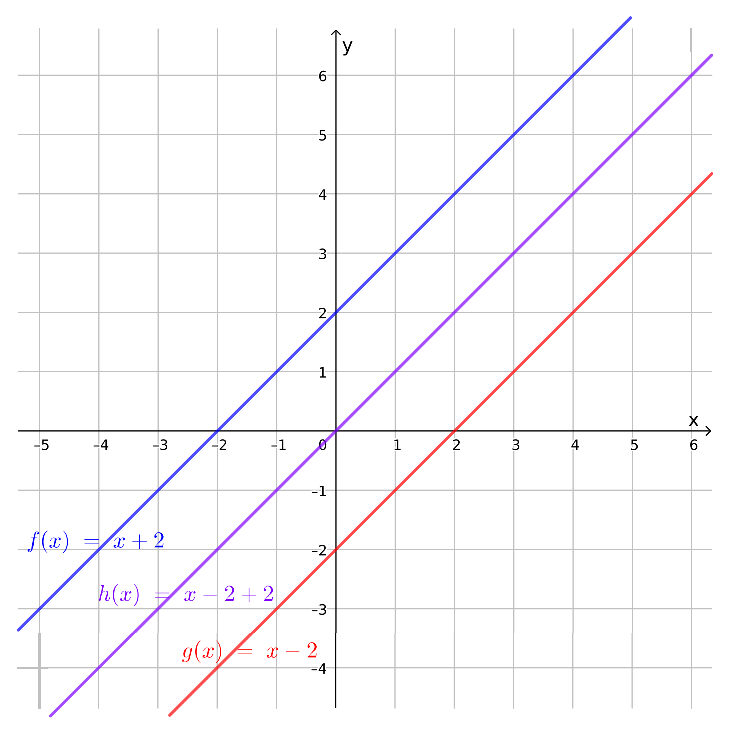
\includegraphics[width=8cm]{./cap_funcao/figs/funcao_composta}}
    \caption{Composta das funções $f$ e $g$}
  \end{figure}

\end{exem}

\newpage
 \section{Mudando os gráficos das funções}

 \subsection{Translação do gráfico das funções}

 Dados $A, B \subset \R$ e uma função $f(x): A \to B$, definimos a função translação de $f$ no eixo $y$, pela função $g(x): A \to B$, dada por \destaque{g(x)= f(x) + c}, onde $c \in \R$ é uma constante.

 \begin{exem}
  Considere a função $f(x): \R \to \R$, dada por $f(x)= x^2$. Defina as seguintes funções $g: \R \to \R$ dada por $g(x)= f(x) + 2= x^2 + 2$, e $h: \R \to \R$ dada por $h(x)= f(x) - 2= x^2 - 2$, observe na seguinte figura como estas translações alteram o gráfico da função $f$, note a função $g$ carregou o gráfico da $f$ duas unidades ``para cima'' no eixo $y$, já a função $h$ carregou o gráfico da $f$ duas unidades ``para baixo'' no eixo $y$.

 \begin{figure}[H]
   \fbox{\subfigure[Gráficos das funções $f$ e $g$]{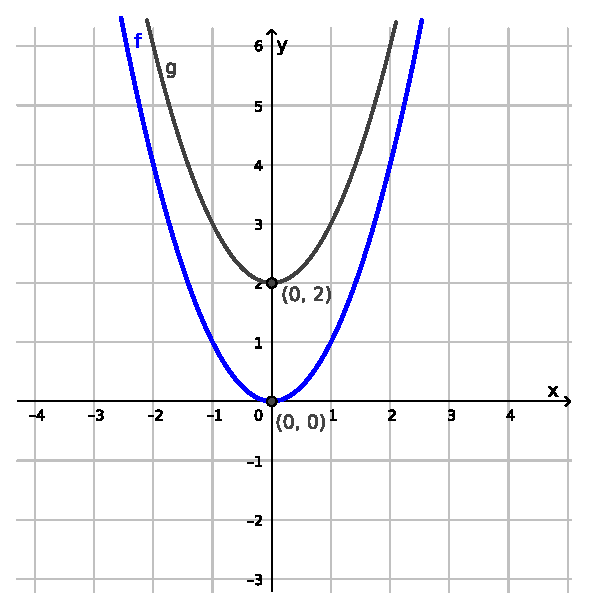
\includegraphics[width=7cm,height=6cm]{./cap_funcao/figs/translacaomais2}}}
   \fbox{\subfigure[Gráficos das funções $f$ e $h$]{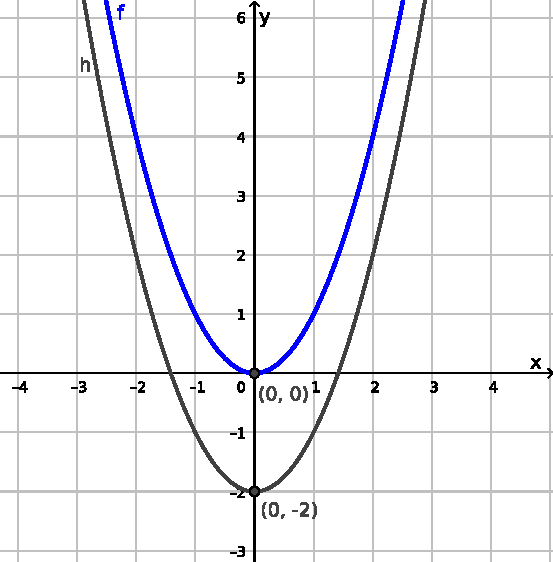
\includegraphics[width=7cm,height=6cm]{./cap_funcao/figs/translacaomenos2}}}
\caption{Translação no eixo $y$}
  \end{figure}

 \end{exem}

  Dados $A, B \subset \R$ e uma função $f(x): A \to B$, definimos a função translação de $f$ no eixo $x$, pela função $g(x): A \to B$, dada por \destaque{g(x)= f(x + c)}, onde $c \in \R$ é uma constante.

 \begin{exem}
  Considere a função $f(x): \R \to \R$, dada por $f(x)= x^2$. Defina as seguintes funções $g: \R \to \R$ dada por $g(x)= f(x + 2)= (x+2)^2$, e $h: \R \to \R$ dada por $h(x)= f(x-2)= (x-2)^2$, observe na seguinte figura como estas translações alteram o gráfico da função $f$, note a função $g$ carregou o gráfico da $f$ duas unidades ``para à esquerda'' no eixo $x$, já a função $h$ carregou o gráfico da $f$ duas unidades ``para à direita'' no eixo $x$.

 \begin{figure}[H]
   \fbox{\subfigure[Gráficos das funções $f$ e $g$]{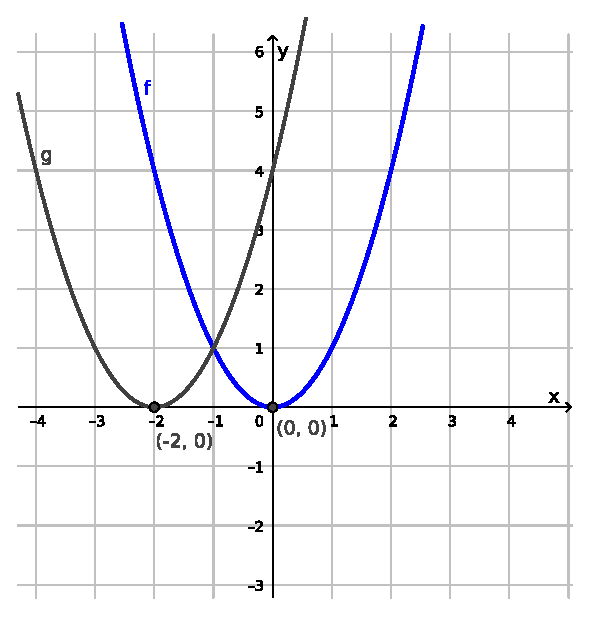
\includegraphics[width=7cm,height=6cm]{./cap_funcao/figs/translacaoXmais2}}}
   \fbox{\subfigure[Gráficos das funções $f$ e $h$]{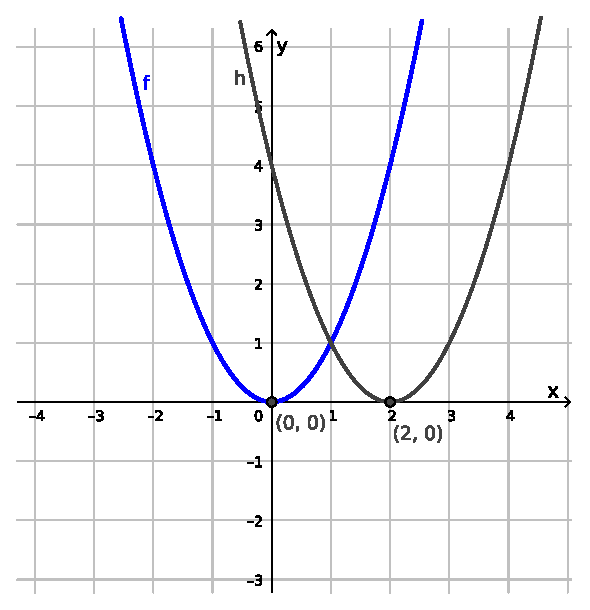
\includegraphics[width=7cm,height=6cm]{./cap_funcao/figs/translacaoXmenos2}}}
\caption{Translação no eixo $x$}
  \end{figure}

 \end{exem}

 \subsection{Reflexão do gráfico das funções}

 Dados $A, B \subset \R$ e uma função $f(x): A \to B$, definimos a função reflexão de $f$ no eixo $x$, pela função $g(x): A \to B$, dada por \destaque{g(x)= -f(x)}.

 \begin{exem}
  Considere a função $f(x): \R \to \R$, dada por $f(x)= x^2$. Defina a função $g: \R \to \R$ dada por $g(x)=-f(x)= -x^2$, note que $g$ é por definição a reflexão da função $f$ em torno do eixo $x$, como pode ser visto pela figura:

\begin{figure}[H]
   \centering
   \fbox{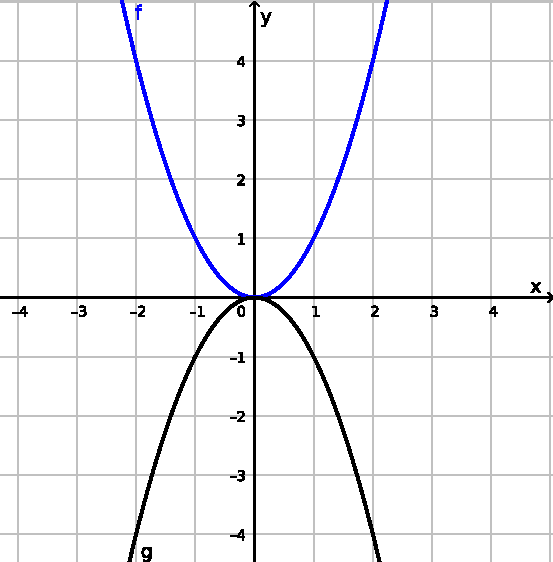
\includegraphics[width=7cm]{./cap_funcao/figs/reflexaoemX}}
   \caption{Reflexão no eixo $x$}
  \end{figure}

 \end{exem}


 Dados $A, B \subset \R$ e uma função $f(x): A \to B$, definimos a função reflexão de $f$ no eixo $y$, pela função $g(x): A \to B$, dada por \destaque{g(x)= f(-x)}.

 \begin{exem}
  Considere a função $f(x): \R \to \R$, dada por $f(x)= x^3$. Defina a função $g: \R \to \R$ dada por $g(x)=f(-x)= (-x)^3$, note que $g$ é por definição a reflexão da função $f$ em torno do eixo $y$, como pode ser visto pela figura:

\begin{figure}[H]
   \centering
   \fbox{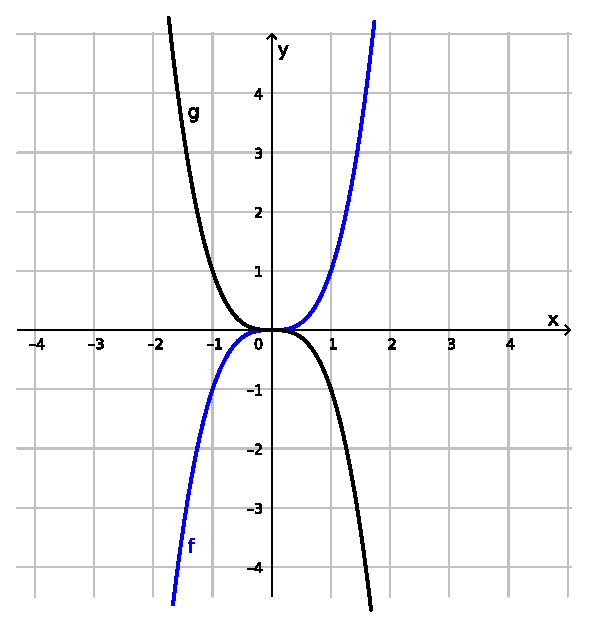
\includegraphics[width=7cm]{./cap_funcao/figs/reflexaoemY}}
   \caption{Reflexão no eixo $y$}
  \end{figure}

 \end{exem}

 Resumindo, dados $A, B \subset \R$, uma função $f(x): A \to B$, e uma constante $c \in \R$ obtemos as seguintes funções $g: A \to B$:
  \begin{table}[H]
 \centering
 \begin{tabular}{|c|c|} \hline
 \rowcolor{cinza}
  Mudança & Função \\\hline
  Translação no eixo $y$ & $g(x)= f(x)+ c$ \\\hline
  Translação no eixo $y$ & $g(x)= f(x)- c$ \\\hline
  Translação no eixo $x$ & $g(x)= f(x+ c)$ \\\hline
  Translação no eixo $x$ & $g(x)= f(x- c)$ \\\hline
  Reflexão no eixo $x$ & $g(x)= -f(x)$ \\\hline
  Reflexão no eixo $y$ & $g(x)= f(-x)$ \\\hline
 \end{tabular}
\end{table}

 \section{Exercícios}
  \begin{exer}
  (UFES) Uma fábrica de papel e celulose possui uma plantação de $100000$ pés de eucalipto em sua área de plantio comercial. A fábrica pretende explorar essa área, derrubando $2000$ pés de eucalipto por dia e, ao mesmo tempo, fazendo o plantio de $m$ pés de eucalipto por dia. Dessa forma, a fábrica espera contar com pelo menos $110000$ pés de eucalipto no prazo de $360$ dias. Para atingir esta meta, o valor mínimo de $m$ deverá ser:
  \begin{enumerate}[a)]
  \item $2025$
  \item $2028$
  \item $2026$
  \item $2029$
  \item $2027$
  \end{enumerate}
  \end{exer}
 
 \begin{exer}
 Uma bolsa de valores tinha um preço de R\$ $42,00$ quando sofreu uma queda de R\$$2,50$ por dia, durante $5$ dias seguidos.
  \begin{enumerate}[a)]
  \item Qual é a função que representa a queda do valor dessa ação em função do dia?
  \item Represente, no plano cartesiano, os pontos correspondentes a esses $5$ dias e o segmento de reta que passa por esses pontos.
  \end{enumerate}
  \end{exer}
  
  \begin{exer}
  Um táxi, realizando uma corrida, cobra uma taxa fixa denominada bandeira de R\$$3,50$ e R\$$0,80$ por quilômetro rodado.
  Com base nesses dados, determine:
  \begin{enumerate}[a)]
  \item A função que representa o valor pago por uma corrida de $x$ quilômetros.
  \item Quantos quilômetros foram rodados se a conta foi de R\$ $17,10$.
  \end{enumerate}
  \end{exer}
  
  \begin{exer}
  Para cercar um terreno, tem-se duas opções:
  1ª) Taxa de entrega no local R\$ $100,00$ e R\$$12,00$ o metro linear de cerca.
  2ª) Taxa de entrega no local R\$ $80,00$ e R\$ $15,00$ o metro linear de cerca.
  \begin{enumerate}[a)]
  \item Represente o custo de cada opção para $x$ metros de cerca.
  \item Qual das duas opções é mais vantajosa para $140$m de perímetro.
  \end{enumerate}
  \end{exer}
  
  \begin{exer}
  No Brasil, o sistema de numeração de sapatos ou tênis é baseado na fórmula $N(p)= \frac{5p + 28}{4}$, que indica o valor aproximado do número do calçado $N$ em função do comprimento $p$, em centímetros do pé da pessoa. Determine o número do sapato ou tênis que uma pessoa deve comprar se, ao medir o comprimento de seu pé obteve:
  \begin{enumerate}[a)]
  \item $22,8$ cm
  \item $24$ cm
  \item $26,4$ cm
  \end{enumerate}
  \end{exer}
  
  \begin{exer}
  (CONSULPLAN - 2010) Sejam os conjuntos $A = \{- 3, - 1, 1, 3, 5, 7\}$ e $B = \{- 4, -2, 0, 2, 4\}$. É correto afirmar:
  \begin{enumerate}[a)]
  \item $f(x) = x + 1$ é uma função de A em B.
  \item $f(x) = 2x + 5$ é uma função de B em A.
  \item $f(x) = 2x - 8$ é uma função de A em B.
  \item $f(x) = x + 3$ é uma função de B em A.
  \item $f(x) = x^2 + 2x - 3$ é uma função de B em A.
 \end{enumerate}
  \end{exer}
  
  \begin{exer}
  (FEPESE - 2017) Uma empresa farmacêutica testou um novo remédio em um grupo de pessoas. Todas tomaram o remédio no mesmo dia, no mesmo momento. Duas pessoas apresentaram reação alérgica no mesmo dia da ingestão do remédio. De fato, a empresa verifica que o número de pacientes que apresentaram reação alérgica ao remédio é dado pela função $r(t) = a t + b$, onde $t$ é o tempo em dias a partir da ingestão do remédio, e $a= 1$ e $b$ são números reais. Se após $3$ dias cinco pessoas apresentaram reação alérgica, quantas pessoas apresentaram reação alérgica após $6$ dias?
 \begin{enumerate}[a)]
  \item $14$.
  \item $12$.
  \item $10$.
  \item $8$.
  \item $6$.
 \end{enumerate}
  \end{exer}
  
  \begin{exer}
  (FEPESE - 2017) Em um shopping, o estacionamento é gratuito pela primeira hora. A segunda hora (ou fração desta) custa R\$ 2,50. A terceira hora (ou fração) custa R\$ 2,75. A quarta hora (ou fração) custa R\$ 3,00 e assim sucessivamente.

 O custo de deixar um carro neste estacionamento por 14 horas e meia é:
 \begin{enumerate}[a)]
  \item Mais do que R\$ 90,00.
  \item Mais do que R\$ 85,00 e menos que R\$ 90,00.
  \item Mais do que R\$ 80,00 e menos que R\$ 85,00.
  \item Mais do que R\$ 75,00 e menos que R\$ 80,00.
  \item Menos que R\$ 75,00.
 \end{enumerate}
  \end{exer}
  
  \begin{exer}
  (FEPESE - 2017) Uma função $f$ definida nos números reais é dita injetiva se $x \neq y$, então $f(x) \neq f(y)$.

Considere as afirmativas abaixo:
\begin{enumerate}[1.]
 \item A função $f$:  dada por $f(x) = x^2$ é injetiva.

 \item Se $f$ é uma função tal que $f(x) = f(y)$ implica que $x = y$, então, $f$ é injetiva.

 \item A função $f$:  dada por $f(x) = -2x + 5$ é injetiva.
 \end{enumerate}
 Assinale a alternativa que indica todas as afirmativas corretas.
 \begin{enumerate}[a)]
 \item É correta apenas a afirmativa 3.
 \item São corretas apenas as afirmativas 1 e 2.
 \item São corretas apenas as afirmativas 1 e 3.
 \item São corretas apenas as afirmativas 2 e 3.
 \item São corretas as afirmativas 1, 2 e 3.
 \end{enumerate}
  \end{exer}
  
  \begin{exer}
  (FEPESE - 2017) Denotamos por $\R$ o conjunto dos números reais. Convencionamos nesta questão que uma função $f : \R \rightarrow \R$ é crescente se $x < y$ implica que $f(x) < f(y)$.

Considere as afirmativas abaixo:
\begin{enumerate}[1.]
\item A função $f:\R \rightarrow \R$, dada por $f(x) = -2x + 25$ é crescente.
\item Se $f$ é tal que $f(x) \geqslant f(y)$ implica $x \geqslant y$ então f é crescente.
\item A função $f: \R \rightarrow \R$ dada por $f(x) = x^2$  é crescente.
\end{enumerate}

Assinale a alternativa que indica todas as afirmativas corretas.

\begin{enumerate}[a)]
 \item É correta apenas a afirmativa 1.
 \item É correta apenas a afirmativa 2.
 \item É correta apenas a afirmativa 3.
 \item São corretas apenas as afirmativas 1 e 2.
 \item São corretas apenas as afirmativas 2 e 3.
\end{enumerate}
  \end{exer}
  
  \begin{exer}
  (FEPESE - 2010) Considere a função $f: \R \rightarrow \R$, definida por
\begin{equation}
f(x)= \frac{1}{\sqrt{x^2 - 1}}
\end{equation}
Assinale a alternativa que indica \textbf{corretamente} o domínio dessa função.
\begin{enumerate}[a)]
\item $\{x \in \R \mid x \neq 1\}$;
\item $\{x \in \R \mid x < -1\} \cup \{x \in \R \mid x > 1\}$;
\item $\{x \in \R \mid x \leqslant -1\} \cup \{x \in \R \mid x \geqslant 1\}$;
\item $\{x \in \R \mid x > -1\} \cup \{x \in \R \mid x < 1\}$;
\item $\{x \in \R \mid x \geqslant -1\} \cup \{x \in \R \mid x \leqslant 1\}$;
\end{enumerate}
  \end{exer}
  
  \begin{exer}
  (Sociesc - 2009) Uma empresa de telefonia celular lançou o seguinte plano de pagamento: uma tarifa mensal fixa de R\$ 25,00 e R\$ 0,50 por minuto usado em ligações locais. Paulo, pensando em fazer este plano de pagamento, perguntou ao vendedor quanto pagaria em um mês que ele usasse o celular durante 2,5 horas com ligações locais. A resposta que o vendedor deu foi:
 \begin{enumerate}[a)]
  \item R\$ 100,00
  \item R\$ 87,50
  \item R\$ 69,00
  \item R\$ 26,25
 \end{enumerate}
  \end{exer}
  
  \begin{exer}
  (Sociesc - 2009) A turma de enfermagem resolveu guardar dinheiro para o pagamento da sua festa de formatura. Para isso, foi feita uma aplicação financeira que obedece a seguinte equação:
\begin{equation}
T = 4.000 + 150x ,
\end{equation}
  onde $T$ é o saldo total e $x$ é o tempo em meses. Sendo assim, o tempo para que o saldo total seja R\$ 10.000,00 será:
  \begin{enumerate}[a)]
  \item 32 meses
  \item 50 meses
  \item 60 meses
  \item 40 meses
 \end{enumerate}
  \end{exer}
  
  \begin{exer}
  (Sociesc - 2010) O valor total cobrado por um eletricista consiste em uma taxa fixa, que é de R\$ 35,00, mais uma quantia que depende da quantidade de fio utilizada por ele no serviço executado. Observando a tabela abaixo, que mostra alguns orçamentos feitos por este eletricista, pode-se afirmar que para um serviço que necessita de 21 metros de fio, o valor total do serviço executado por ele será de:

  \begin{table}[H]
  \centering
 \begin{tabular}{|c|c|} \hline
  \multicolumn{1}{|c|}{\textbf{Quantidade de fio
(metros)}} & \multicolumn{1}{|c|}{\textbf{Valor total do serviço
(R\$)}} \\ \hline
 6 & 53,00 \\ \hline
 8 & 59,00 \\ \hline
 12 & 71,00 \\ \hline
 \end{tabular}
\end{table}

  \begin{enumerate}[a)]
  \item R\$ 91,00
  \item R\$ 90,00
  \item R\$ 98,00
  \item R\$ 94,00
  \item R\$ 93,00
 \end{enumerate}
  \end{exer}
  
  \begin{exer}
  (Sociesc - 2010) Uma empresa que faz fotocopia criou um plano para o pagamento das cópias. O plano consiste em uma taxa fixa (mensal) de R\$ 50,00 e mais R\$ 0,07 por cópia. O número mínimo de cópias que devem ser tiradas em um mês, por um só cliente, para que o preço total ultrapasse R\$ 99,00, é:
  \begin{enumerate}[a)]
  \item 701
  \item 700
  \item 710
  \item 670
  \item 680
 \end{enumerate}
  \end{exer}
  
  \begin{exer}
  (Sociesc - 2010) Uma empresa de componentes eletrônicos tem, para um de seus componentes, um custo diário de produção dado por $C(x) = x^2 - 120x + 2500$, onde $C(x)$ é o custo em reais e $x$ é o número de unidades fabricadas. O número de componentes eletrônicos que devem ser produzidos diariamente para que o custo seja mínimo é:
 \begin{enumerate}[a)]
  \item 54
  \item 122
  \item 50
  \item 60
  \item 141
 \end{enumerate}
  \end{exer}
  
  \begin{exer}
  (Sociesc - 2010) Uma corrida de táxi inclui uma taxa fixa, denominada bandeirada, e uma parcela que depende da distância percorrida. A bandeirada custa R\$ 5,30 e cada quilômetro rodado custa R\$ 1,20. A distância aproximada percorrida por um passageiro que pagou R\$ 25,30 foi de?
  \begin{enumerate}[a)]
  \item 20 km
  \item 15 km
  \item 16,6 km
  \item 17,6 km
  \item 20,6 km
 \end{enumerate}
  \end{exer}
  
  \begin{exer}
  (Sociesc - 2008) Um reservatório esta sendo esvaziado para limpeza. O seu volume varia com o tempo de acordo com a função $V(t)= 120(20 - t)^2$, onde o volume é dado em litros e o tempo, em minutos. De acordo com esta lei, podemos afirmar que o tempo que o reservatório demora para ficar vazio e a quantidade de litros que são escoados nos primeiros 10 minutos são respectivamente:
  \begin{enumerate}[a)]
  \item 22 horas e 36.000 litros
  \item 20 horas e 36.000 litros
  \item 20 horas e 30.000 litros
  \item 22 horas e 30.000 litros
 \end{enumerate}
  \end{exer}
  
  \begin{exer}
  (UDESC/Fepese - 2009) Considere a função $f: \R \to \R$, definida por:
\begin{equation}
f(x)= \frac{1}{\sqrt{x^2 - 1}}
\end{equation}
 Assinale a alternativa que indica \textbf{corretamente} o domínio dessa função.
 \begin{enumerate}[a)]
 \item $\{x \in \R \mid x \neq 1\}$
 \item $\{x \in \R \mid x < -1\} \cup \{x \in \R \mid x>1\}$
 \item $\{x \in \R \mid x \leq -1\} \cup \{x \in \R \mid x \geq 1\}$
 \item $\{x \in \R \mid x > -1\} \cup \{x \in \R \mid x>1\}$
 \item $\{x \in \R \mid x \geq -1\} \cup \{x \in \R \mid x\leq 1\}$
 \end{enumerate}
  \end{exer}
 
 
 Gabarito: 1 b); 2 a) $f(x)= 42 - 2,50 x$; 2 b) a cargo do leitor; 3 a) $f(x)= 3,50 + 0,80 x$; 3 b) $x= 17 Km$; 4 a) 1ª opção: $f(x)= 100 + 12x$, 2ª opção: $f(x)= 80+15x$; 4 b) 1ª opção; 5 a) $35,5$; 5 b) $37$; 5 c) $40$; 6 d); 7 d); 8 e); 9 d); 10 b); 11 b); 12 a); 13 d); 14 c); 15 a); 16 d); 17 c); 18 b); 19 b).
  


 